
Si bien estas primitivas son fáciles de generar, también son muy simples y nos serán insuficientes si queremos construir escenas más complejas. Como comentamos en la introducción, una de las principales ventajas del uso de ecuaciones implícitas para representar modelos geométricos es la facilidad de combinación de estas primitivas, por ejemplo mediante operaciones booleanas o deformaciones. Sin embargo los sistemas que hacían uso de esta técnica no estaban lo suficientemente estructurados como para permitir aplicar estas operaciones de manera general e intuitiva, haciendo que no se pudieran aplicar de forma local y por tanto no se pudieran generar escenas complejas.\newline


Esto cambió en 1999 con el artículo de B. Wyvill y otros \cite{blobtree}, en el que sugieren usar una estructura de árbol para definir modelos como combinación de otros a través de operaciones básicas. La gran ventaja de este método es que es muy extensible, y además permite ver de forma muy clara la estructura del modelo. En esta sección estudiaremos los principales tipos de estas operaciones.

\subsection{Operaciones booleanas}
Una de las técnicas más útiles para generar nuevas formas a partir de primitivas es la geometría de sólidos constructiva. Por la naturaleza de las SDFs, estas operaciones se implementan fácilmente usando las funciones máximo y mínimo.

\begin{definicion}[Operaciones Booleanas]\label{p:boolean}
    Sean $A$ y $B$ isosuperficies generadas por $\phi$ y $\gamma$ respectivamente. La función $\mu$ define la isosuperficie para las siguientes operaciones.
    \begin{itemize}
        \item \textbf{Unión: } $\mu_{A\cup B}(p) = \Min(\phi(p), \gamma(p))$.
        \item \textbf{Intersección: } $\mu_{A\cap B}(p) = \Max(\phi(p), \gamma(p))$.
        \item \textbf{Diferencia: } $\mu_{A\setminus B}(p) = \Max(\phi(p), -\gamma(p))$.
    \end{itemize}
\end{definicion}

Solo en el caso de la unión se obtiene una SDF exacta, ya que al aplicar la función máximo en el interior de la superficie (donde $\phi(p) < 0$) el resultado puede ser solo una cota inferior de la distancia. En nuestro caso solo estamos interesados en visualizar la frontera de las superficies así que podemos obviar este problema, con la salvedad de que el algoritmo de \textit{spheretracing} requiera de más iteraciones.\newline

Un problema de usar estas transformaciones es que produce discontinuidades en la derivada de la función resultante. Trataremos de evitar esta situación, además de por motivos analíticos, por motivos visuales, ya que esto produce bordes muy acusados en la intersección de ambas superficies. Existen muchas formas de combinar funciones distancia de forma más natural. Usaremos una de las más extendidas, usada por programas de modelado 3D como Blender \cite{repo:blender} o videojuegos como Dreams \cite{game:dreams}, y que ha sido estudiada por Íñigo Quílez en su web \cite{article:smooth}.

\begin{observacion}
    Para mayor claridad del razonamiento, en las figuras se representarán funciones de variable real, a pesar de que nosotros trabajamos en $\R^3$.
\end{observacion}

Explicaremos la técnica poniendo como ejemplo la unión, y al final veremos como la intersección y la diferencia se deducen fácilmente de esta. La idea es, dadas $\phi$ y $\gamma$, añadir una corrección para cada punto a la función mínimo original para que cumpla ciertos requisitos. Por comodidad, definiremos 
\begin{align*}
      \Min_{\phi,\gamma}\colon \R^3 &\to \R,\\
      p &\mapsto \Min(\phi(p),\gamma(p)).
\end{align*}

Llamaremos a la mencionada corrección $\omega_k\colon \R^3\to\R$, donde $k\in \R_0^+$ es un coeficiente que controlará la intensidad del suavizado. Por tanto, la versión suavizada de la función mínimo original será
\begin{align*}
      \smin_{\phi,\gamma}\colon \R^3 &\to \R,\\
      p &\mapsto \Min_{\phi,\gamma}(p) - \omega_k(p).
\end{align*}

Como no queremos que este cambio afecte al algoritmo de \textit{spheretracing}, debemos asegurar que se cumpla $\Min_{\phi,\gamma}(p)\ge \smin_{\phi,\gamma}(p)$, esto es,
\begin{equation*}
\omega_k(p)\ge 0,\ \text{para todo } p\in \R^3,\ \text{para todo } k\in \R^+_0.
\end{equation*}

Si estudiamos cómo se comporta la versión real de la función mínimo en la \autoref{fig:min_real}, vemos que los puntos de conflicto se encuentran cerca de las intersecciones de las gráficas de $\phi$ y $\gamma$, es decir, cuando $\phi$ y $\gamma$ están arbitrariamente cerca. En el resto de puntos no queremos modificar la función original, luego estudiaremos el comportamiento de $\smin$ en el conjunto de entornos de las intersecciones. Usaremos el valor de $k$ para decidir el tamaño de estos entornos, aplicando la corrección únicamente en los puntos del conjunto
\begin{equation*}
    B_{k} = \{p\in\R^3 : |\phi(p)-\gamma(p)| \le k\},
\end{equation*}
de forma que $\omega(p) = 0$ cuando $p\notin B_{k}$.\newline

\begin{figure}[t]
    \centering
    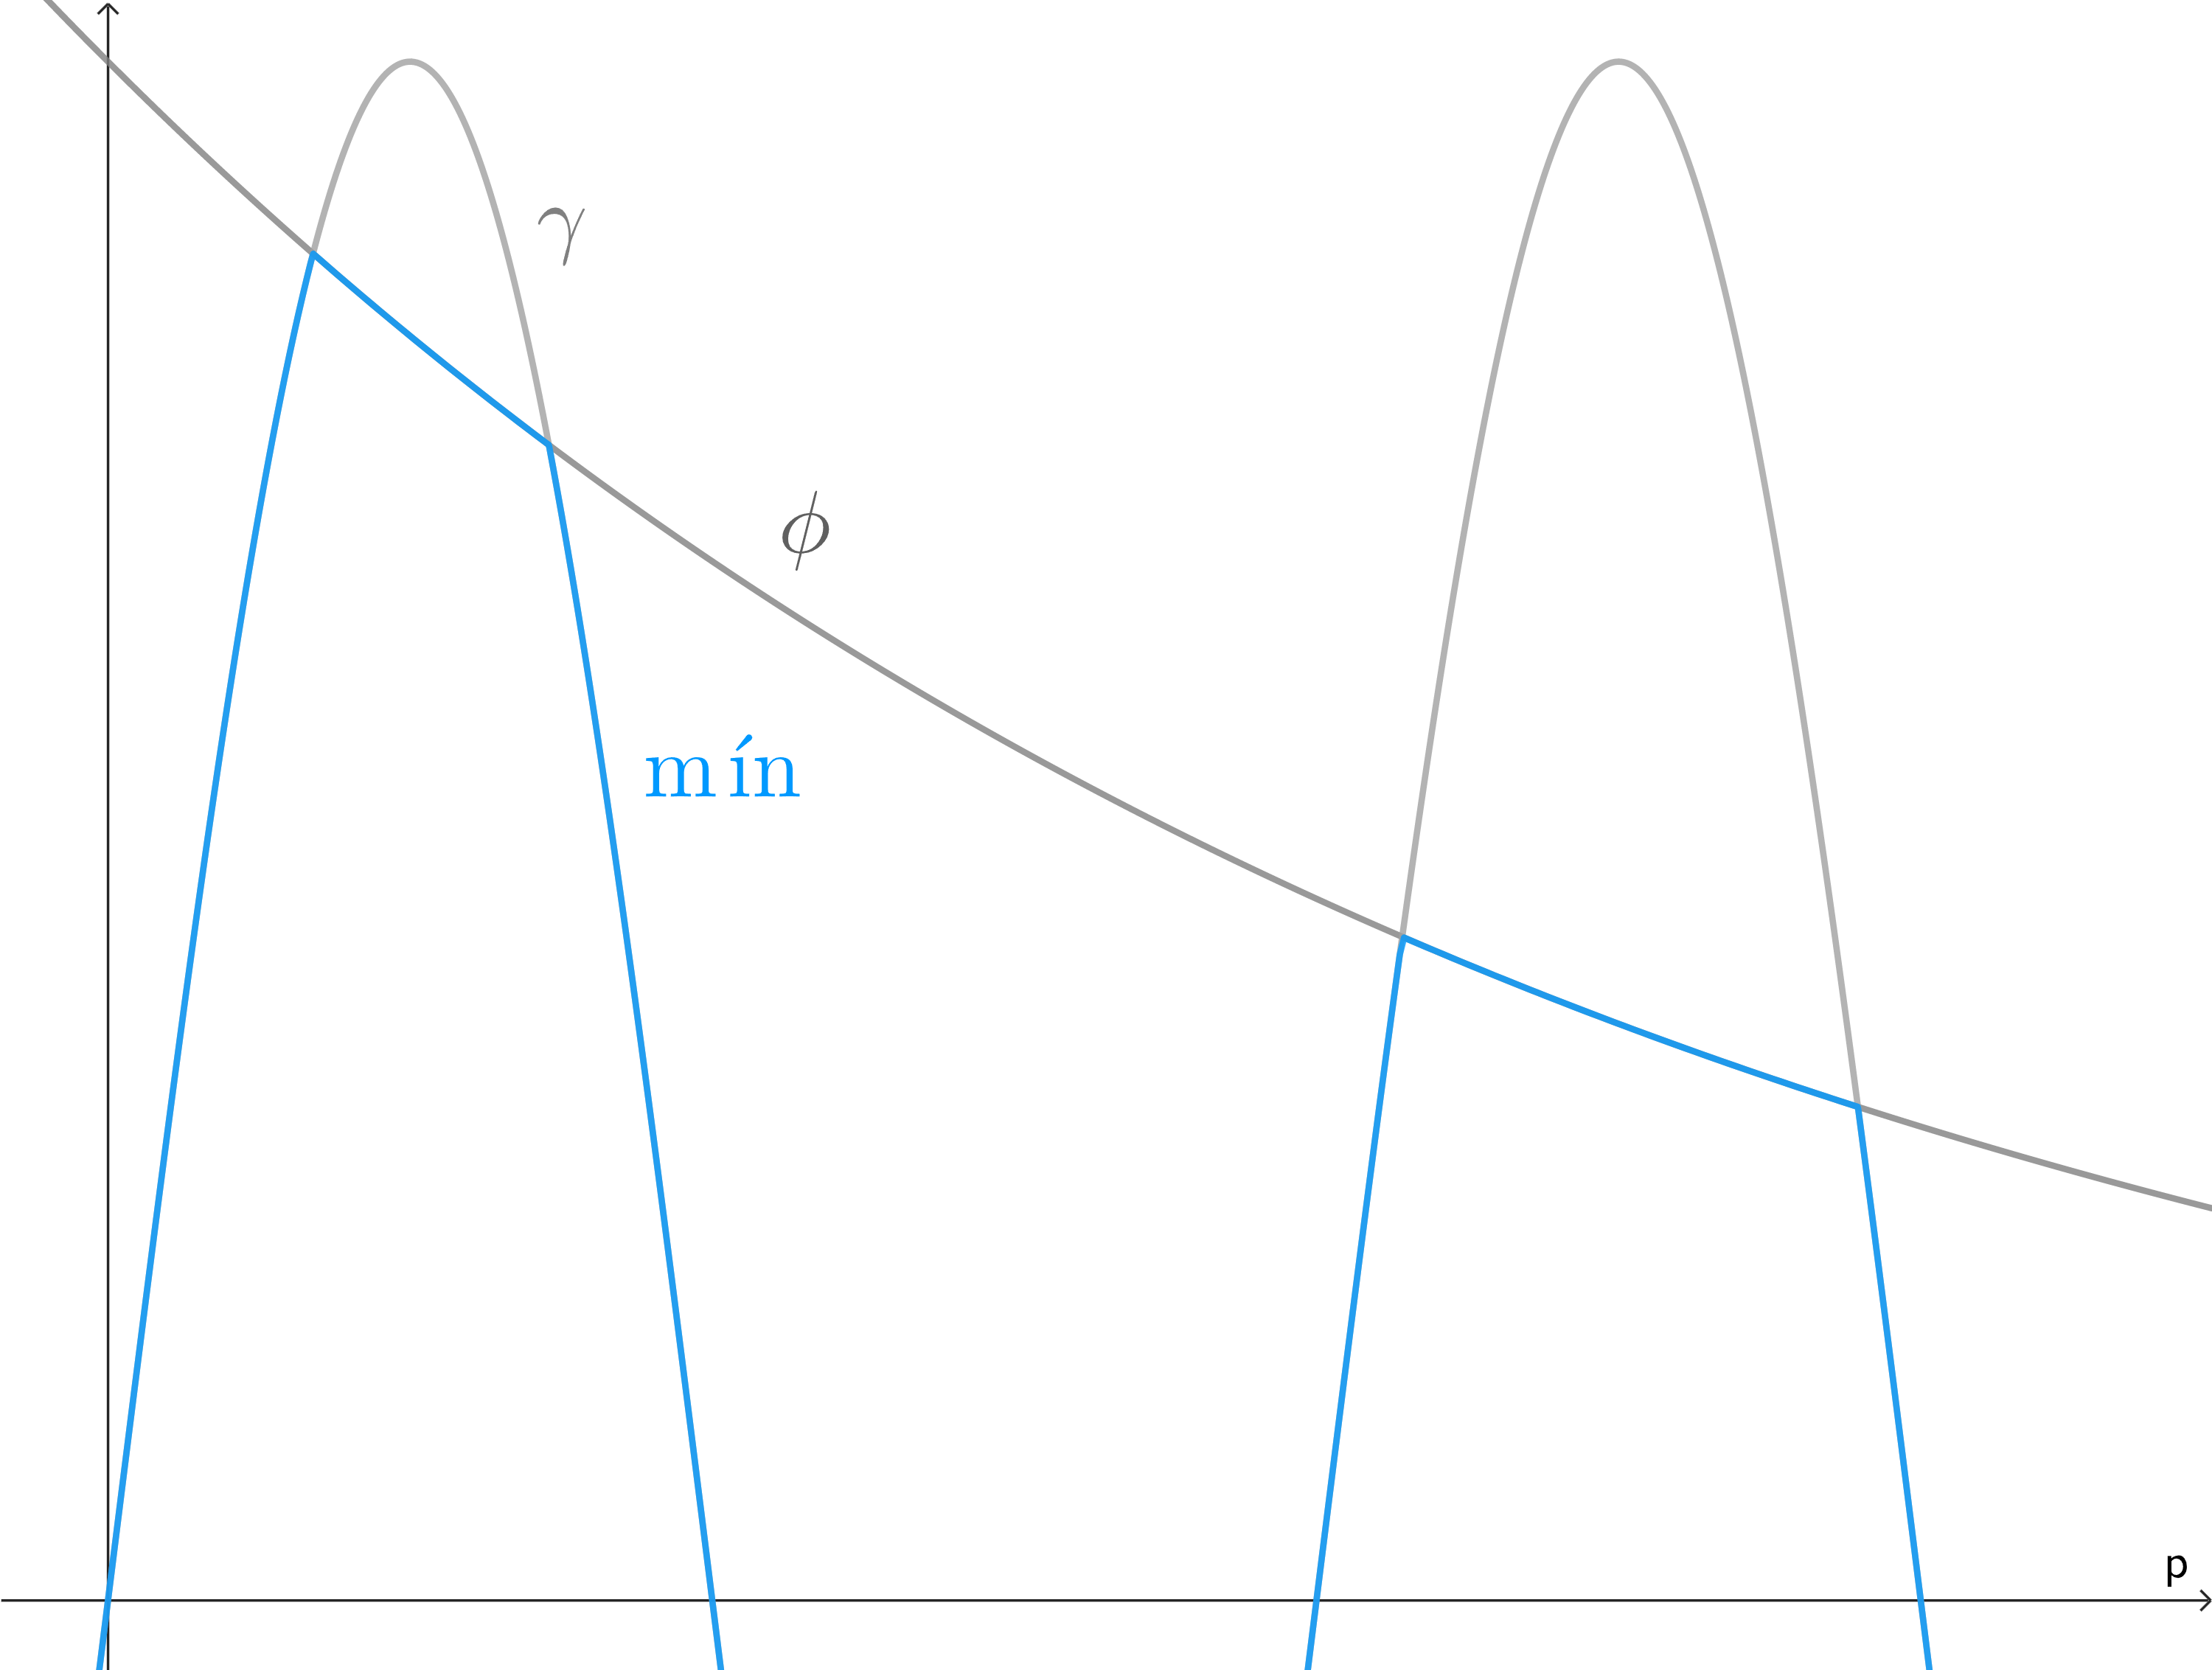
\includegraphics[width=0.75\textwidth]{Plantilla-TFG-master/img/smooth_real.png}
    \caption{Gráfica de $\Min\colon \R\to\R$}
    \label{fig:min_real}
\end{figure}

Para asegurar que $\smin$ sea continua en la frontera de $B_{k}$, imponemos la condición 
\begin{equation*}
    \omega_k(p) = 0,\ \text{para todo } p \in \delta B_{k}.
\end{equation*}
Por otro lado, es lógico que $\omega_k$ tenga su mayor influencia justo en las intersecciones, luego imponemos también 
\begin{equation*}
    \omega_k(c) = s, \text{ donde } c \in I = \{p\in\R^3 : \phi(p) = \gamma(p)\},\ s\in \R.
\end{equation*}

El valor $s$ es el que deberemos ajustar para que $\smin$ cumpla nuestros requisitos. Fijado un $p\in B_{k}$, consideramos una primera aproximación para $\omega_k$ :
\begin{equation*}
    \omega_k(p) = s\left( 1-\frac{|\phi(p)-\gamma(p)|}{k} \right)^n = \begin{cases}
        s\left( 1-\frac{\phi(p)-\gamma(p)}{k}\right)^n,\ \phi(p)>\gamma(p), \\[10pt]
        s\left( 1+\frac{\phi(p)-\gamma(p)}{k}\right)^n,\ \phi(p)\le \gamma(p)\\[10pt]
    \end{cases}  ,\ s\in\R,\ n\in\N,
\end{equation*}
donde hemos añadido el parámetro $n$ para añadir más control sobre el resultado final.\newline 
\begin{figure}[!h]
     \begin{minipage}[c]{0.49\linewidth}
        \centering
        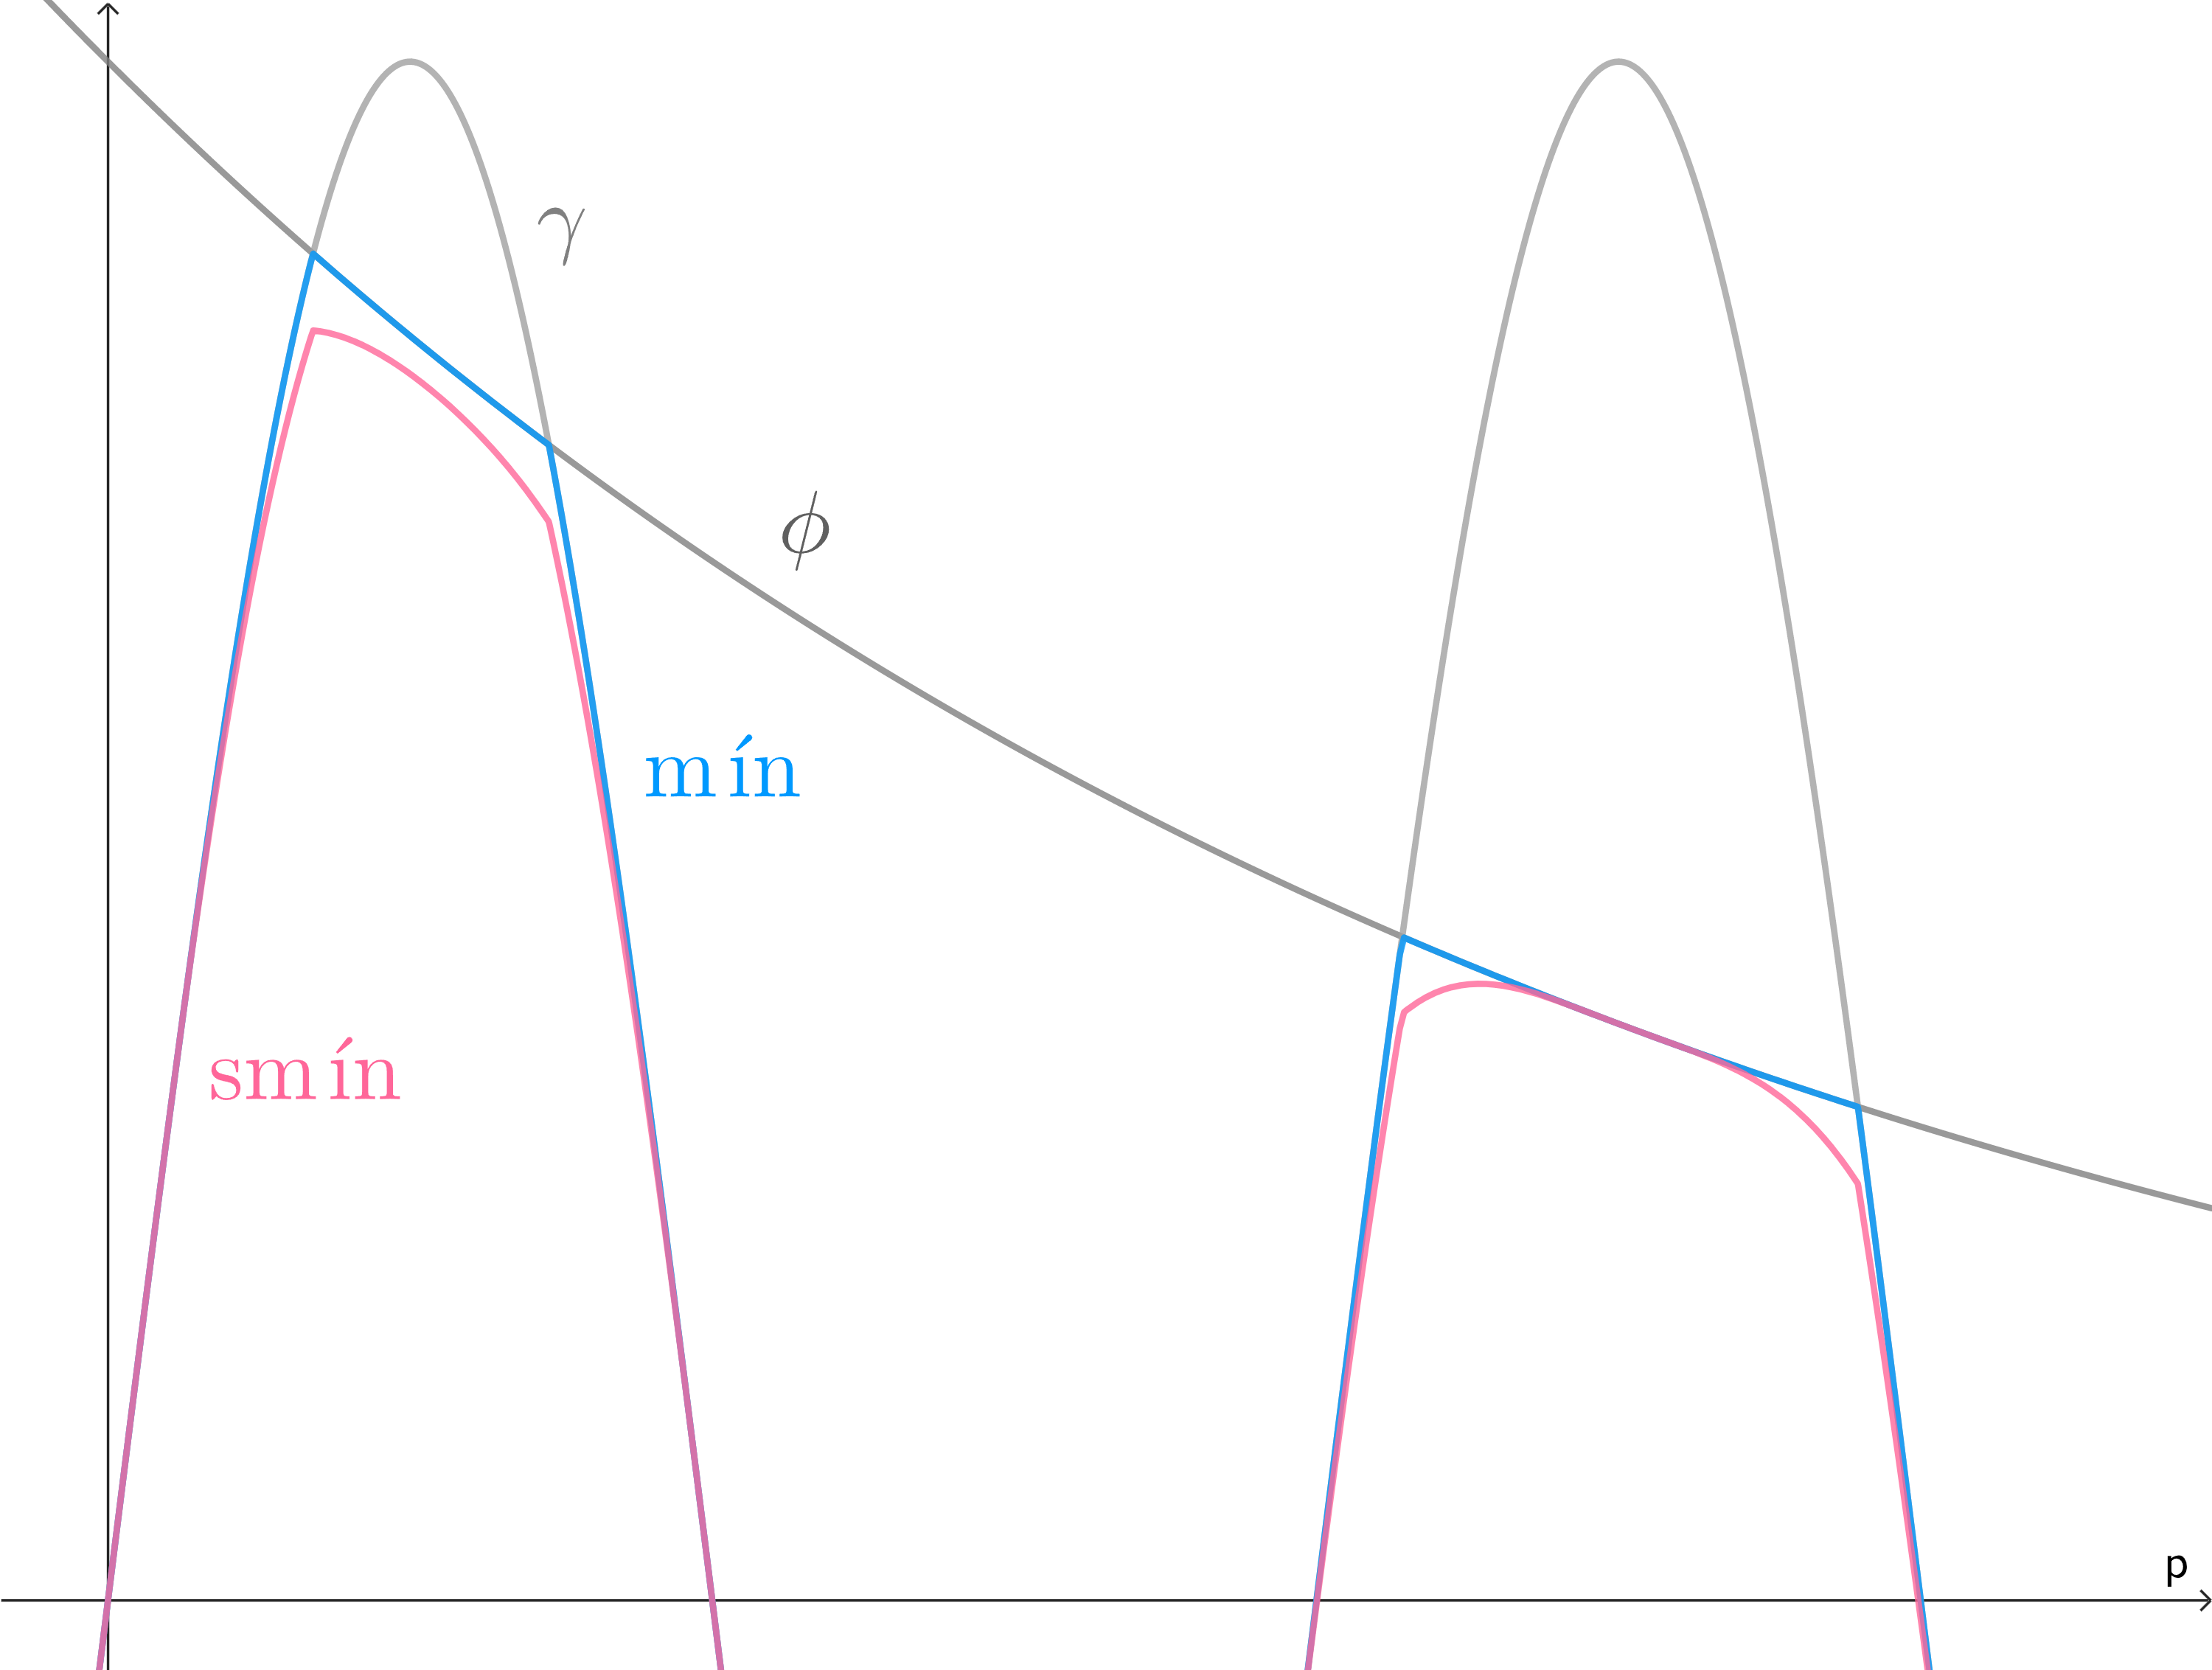
\includegraphics[width=0.95\textwidth]{Plantilla-TFG-master/img/smin_1.png}
        \caption{$k=0.6$}
     \end{minipage}
     \begin{minipage}[c]{0.49\linewidth}
        \centering
        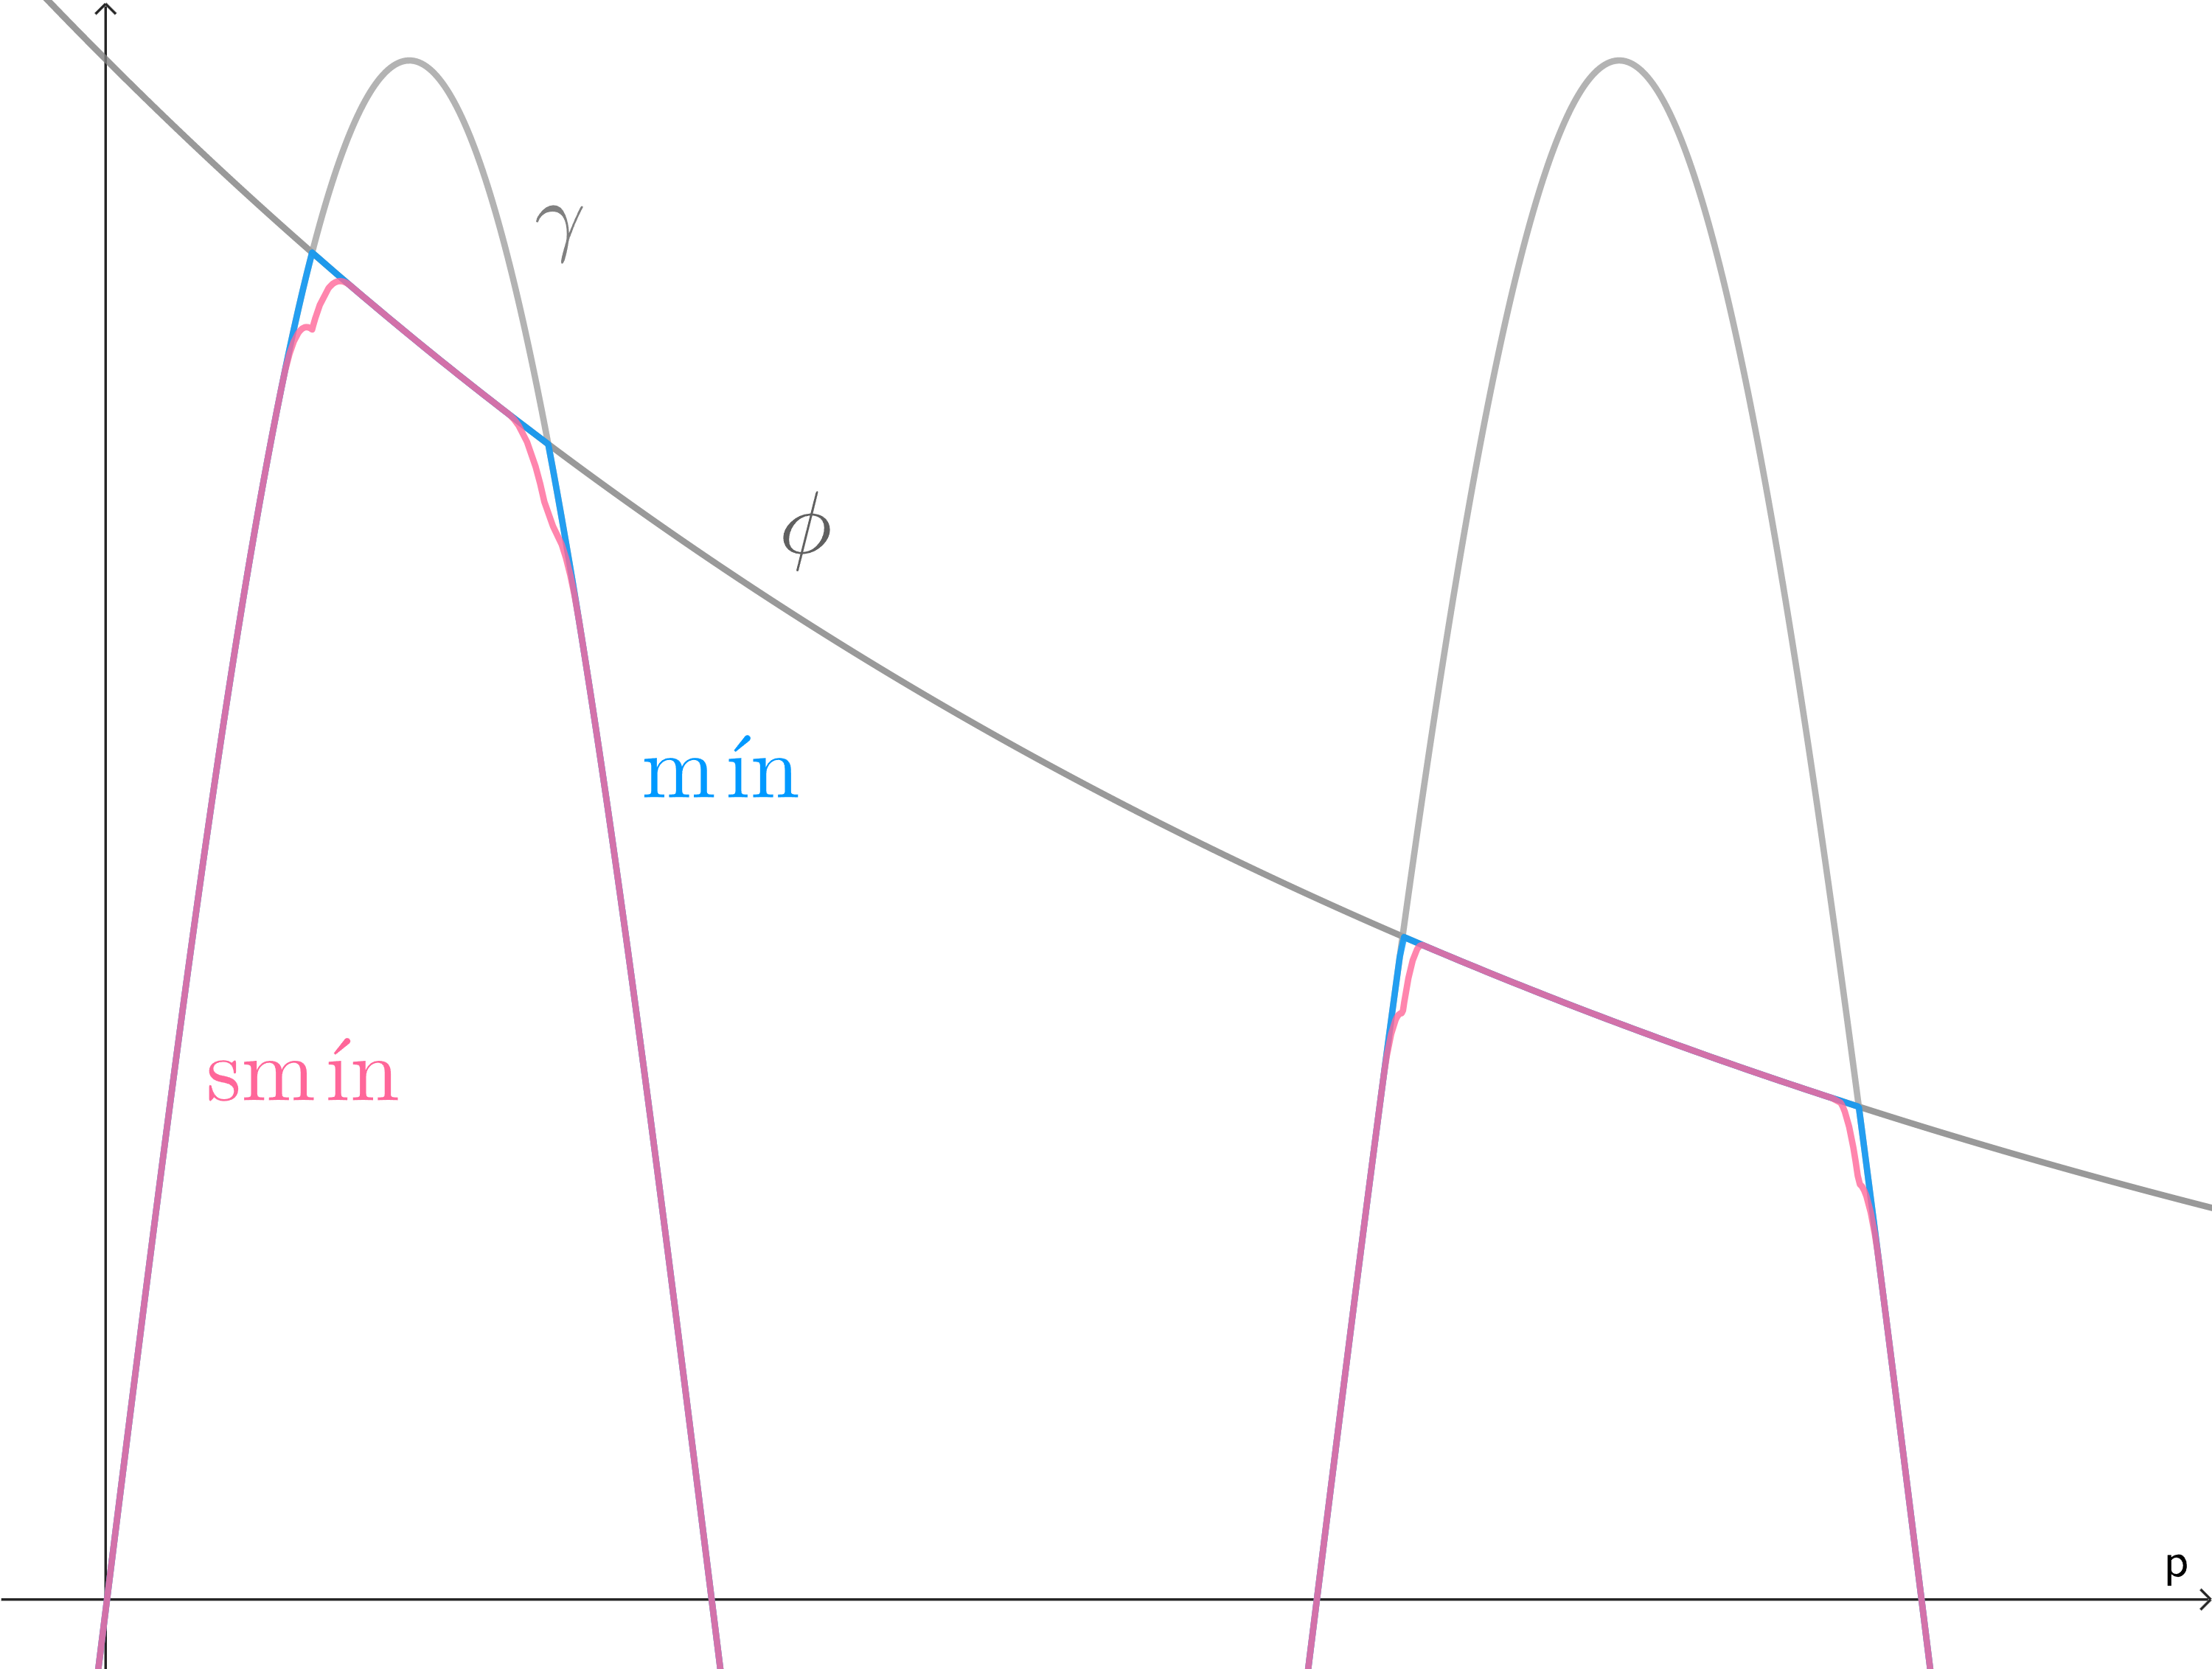
\includegraphics[width=0.95\textwidth]{Plantilla-TFG-master/img/smin_2.png}
        \caption{$k=0.1$}
     \end{minipage}
     \caption{Primera aproximación de $smin(p)$ con $s=0.05$ y $n=2$}
     \label{fig:smooth1}
\end{figure}

Nuestro objetivo es que $\smin$ tenga un aspecto natural y varíe de forma suave. Comprobemos las propiedades que debería cumplir $\smin$ para ser $\mathcal{C}^1$ en cada entorno de $B_k$. Que es continua es evidente:
\begin{equation*}
    \phi(p)=\gamma(p), \text{ luego } \frac{\phi(p)-\gamma(p)}{k} = 0, \text{ y por tanto } \omega_k(p) = s.
\end{equation*}

Otra condición necesaria es que sus derivadas parciales sean continuas. Para todo $i\in \{1,2,3\}$, estas son de la forma
\begin{align*}
    \frac{\partial \smin}{\partial x_i}(p) &= \begin{cases}
        \frac{\partial \gamma}{\partial x_i}(p)+ sn\left(1-\frac{\phi(p)-\gamma(p)}{k}\right)^{n-1}\left(\frac{ \frac{\partial \phi}{\partial p}(p)-\frac{\partial \gamma}{\partial p}(p)}{k}\right),\ \phi(p)>\gamma(p), \\[10pt] 
        \frac{\partial \phi}{\partial x_i}(p)+ sn\left(1-\frac{\phi(p)-\gamma(p)}{k}\right)^{n-1}\left(\frac{ \frac{\partial \phi}{\partial p}(p)-\frac{\partial \gamma}{\partial p}(p)}{k}\right),\ \phi(p)\le\gamma(p).
    \end{cases}
\end{align*}

Por tanto, para comprobar que las parciales son continuas cuando $\phi(p) = \gamma(p)$, para todo $i\in \{1,2,3\}$ imponemos 
\begin{align*}
     \frac{\partial \phi}{\partial x_i} - sn\left(1+\frac{\phi-\gamma}{k}\right)^{n-1}\left(\frac{\frac{\partial \phi}{\partial x_i}-\frac{\partial \gamma}{\partial x_i}}{k}\right) &= \frac{\partial \gamma}{\partial x_i} + sn\left(1-\frac{\phi-\gamma}{k}\right)^{n-1}\left(\frac{\frac{\partial \phi}{\partial x_i}-\frac{\partial \gamma}{\partial x_i}}{k}\right),\\[10pt]
     \cancel{\frac{\partial \phi}{\partial x_i} - \frac{\partial \gamma}{\partial x_i}} &= 2sn\left(1-\frac{\phi-\gamma}{k}\right)^{n-1}\left(\frac{ \cancel{\frac{\partial \phi}{\partial x_i}-\frac{\partial \gamma}{\partial x_i}}}{k}\right),\\[10pt]
     s &= \frac{k}{2n}\left(1-\frac{\phi-\gamma}{k}\right).
\end{align*}

Evaluando en $c\in I$:
\begin{align*}
    s = \frac{k}{2n}\left(1-\frac{\cancelto{0}{\phi(c)-\gamma(c)}}{k}\right), \text{ luego } s = \frac{k}{2n}.
\end{align*}
    
Hemos llegado a la expresión final
\begin{align}
    \label{eq:correccion}
    \omega_k(p) &= \begin{cases}
        \frac{k}{2n}\left( 1-\frac{|\phi(p)-\gamma(p)|}{k} \right)^n,\ &|\phi(p)-\gamma(p)|\le k,\\[10pt]
        0,\ &\text{ otro caso },
    \end{cases}\\[10pt] &= \frac{\Max\left( k - |\phi(p) - \gamma(p)|, 0\right)^n}{2n\cdot k^{n-1}}  ,\ s\in\R,\ n\in\N. 
\end{align}

Podemos observar los resultados en la \autoref{fig:smooth2}. Finalmente, para obtener una versión suavizada del máximo, es fácil comprobar que 
\begin{align*}
      \smax_{\phi,\gamma}\colon \R^3&\to \R,\\
      p &\mapsto -\smin_{-\phi,-\gamma}(p).
\end{align*}

Con estos resultados, para que la transición de una superficie a otra en la \autoref{p:boolean} sea gradual basta con sustituir las versiones clásicas de las funciones máximo y mínimo por las que acabamos de obtener.  
\begin{figure}[!h]
     \begin{minipage}[c]{0.49\linewidth}
        \centering
        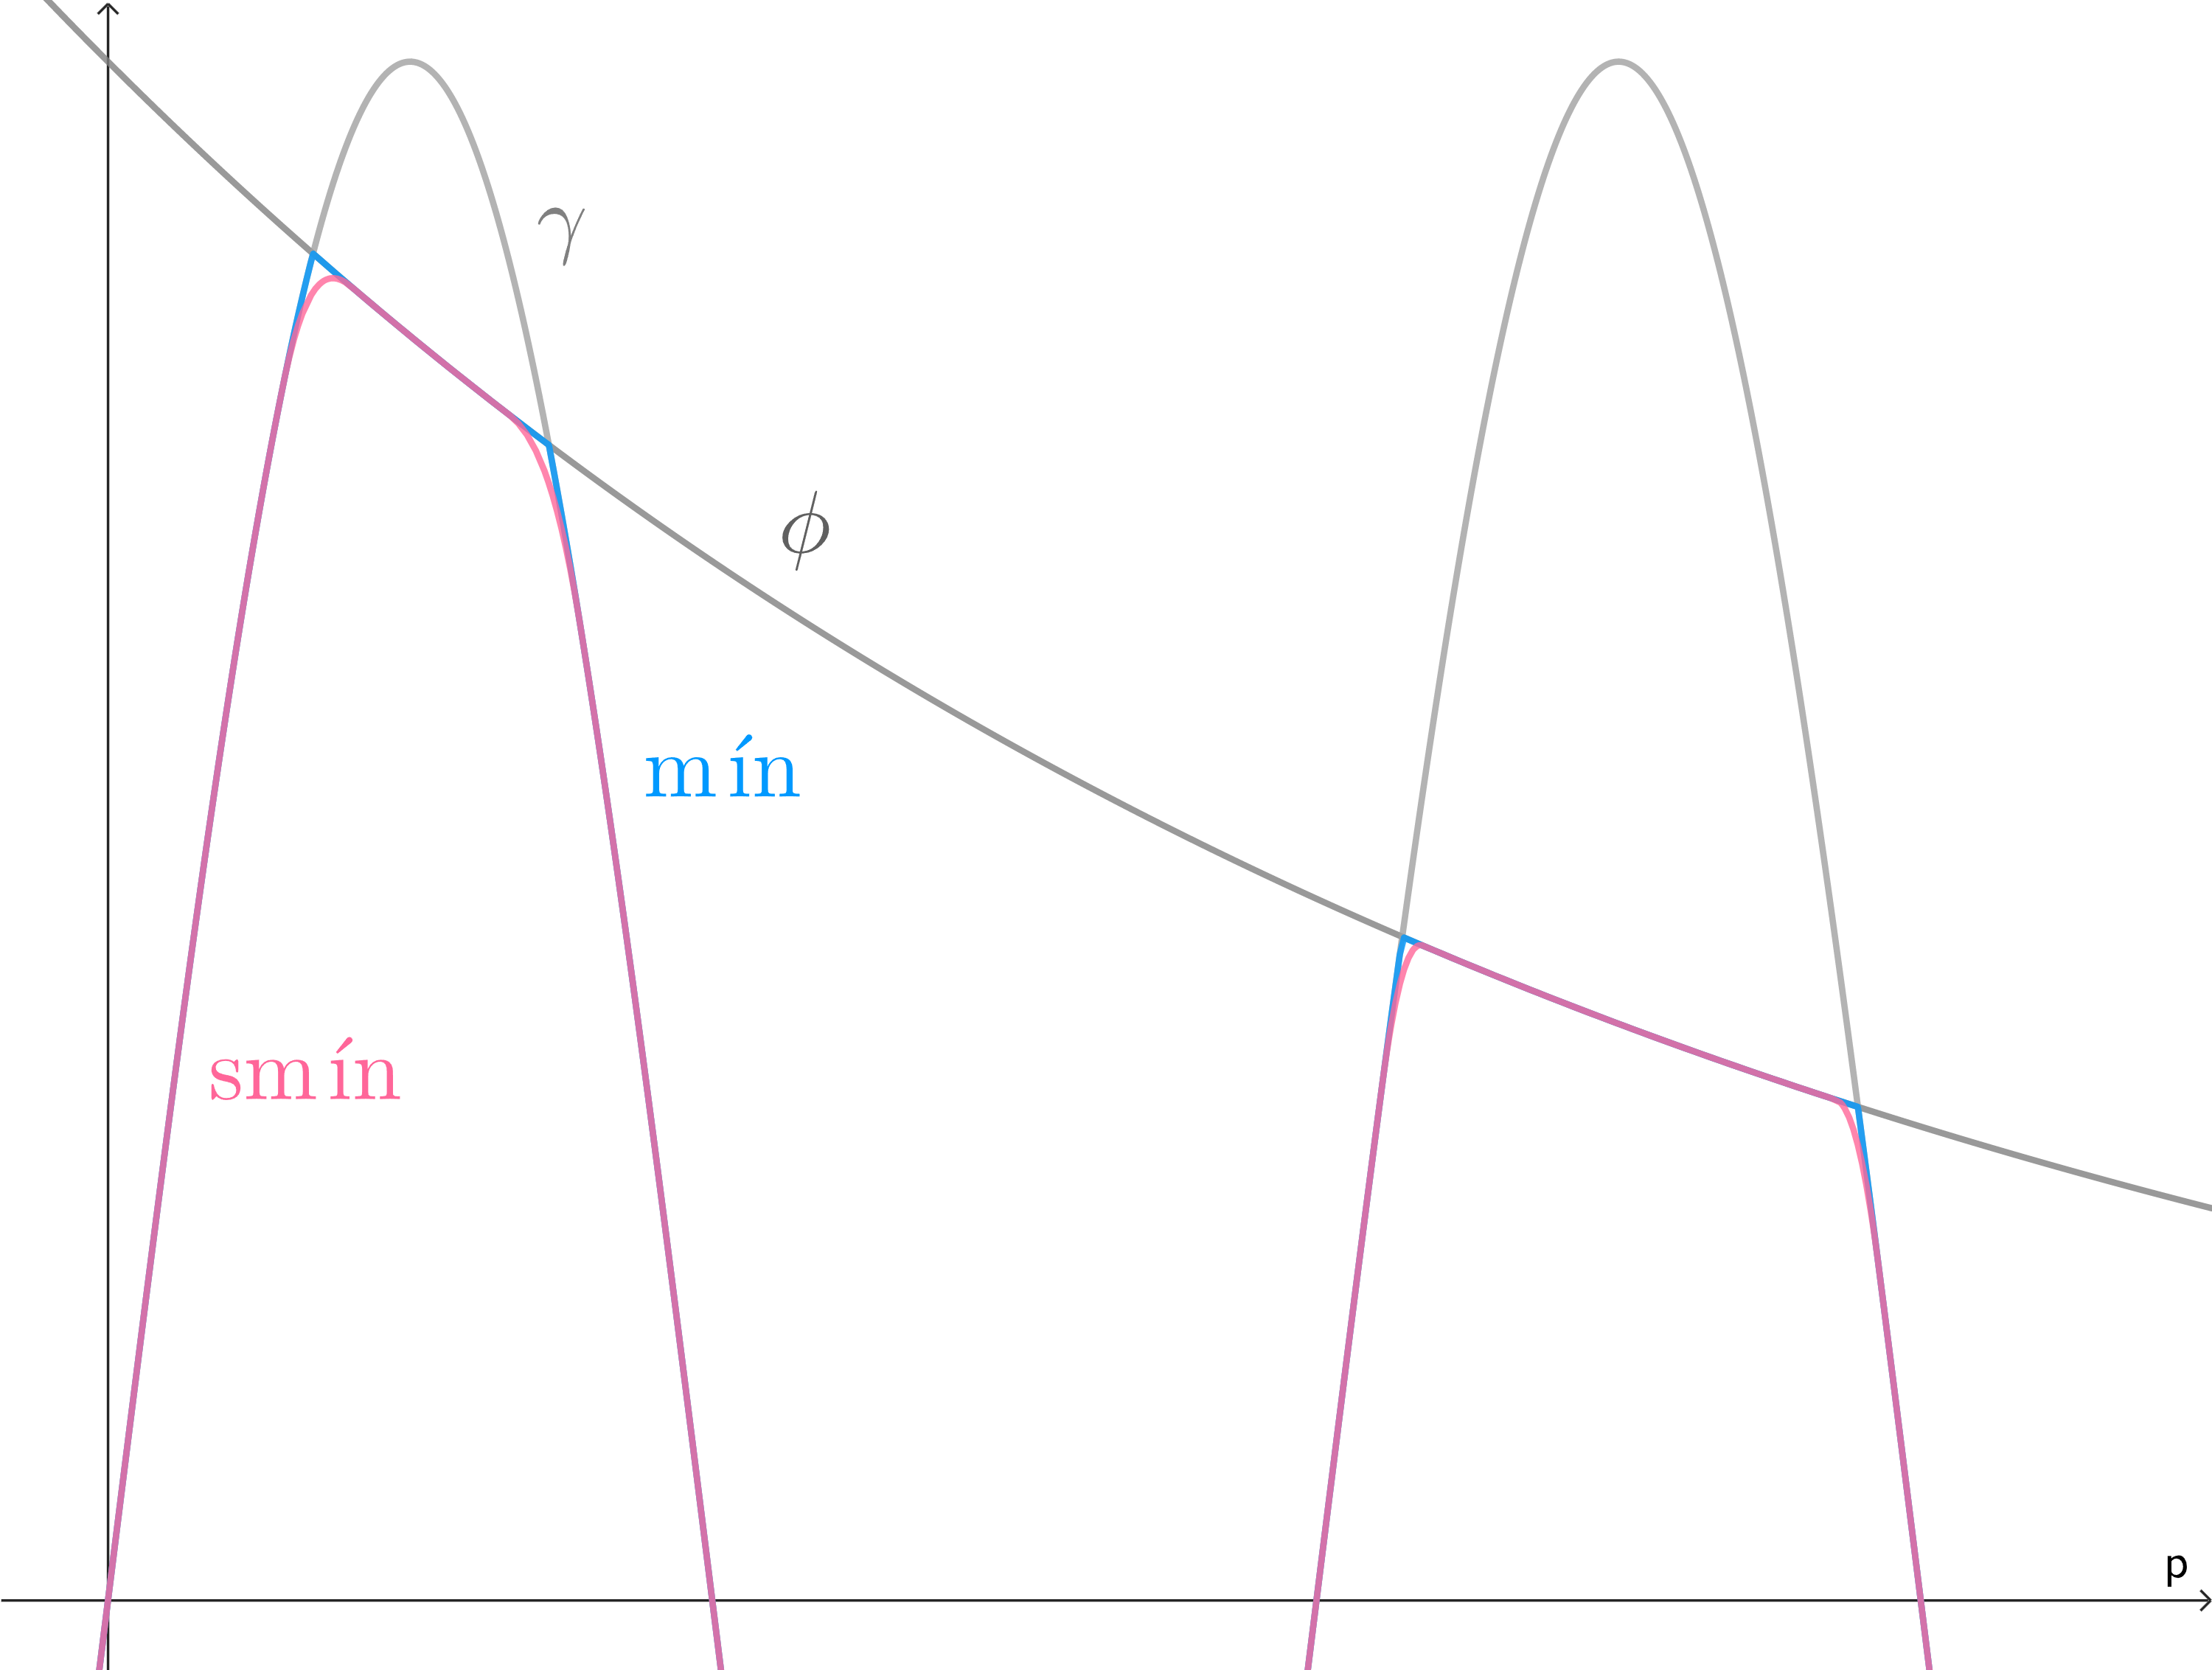
\includegraphics[width=0.95\textwidth]{Plantilla-TFG-master/img/smin_3.png}
        \caption{$k=0.1,\ n=2$}
     \end{minipage}
     \begin{minipage}[c]{0.49\linewidth}
        \centering
        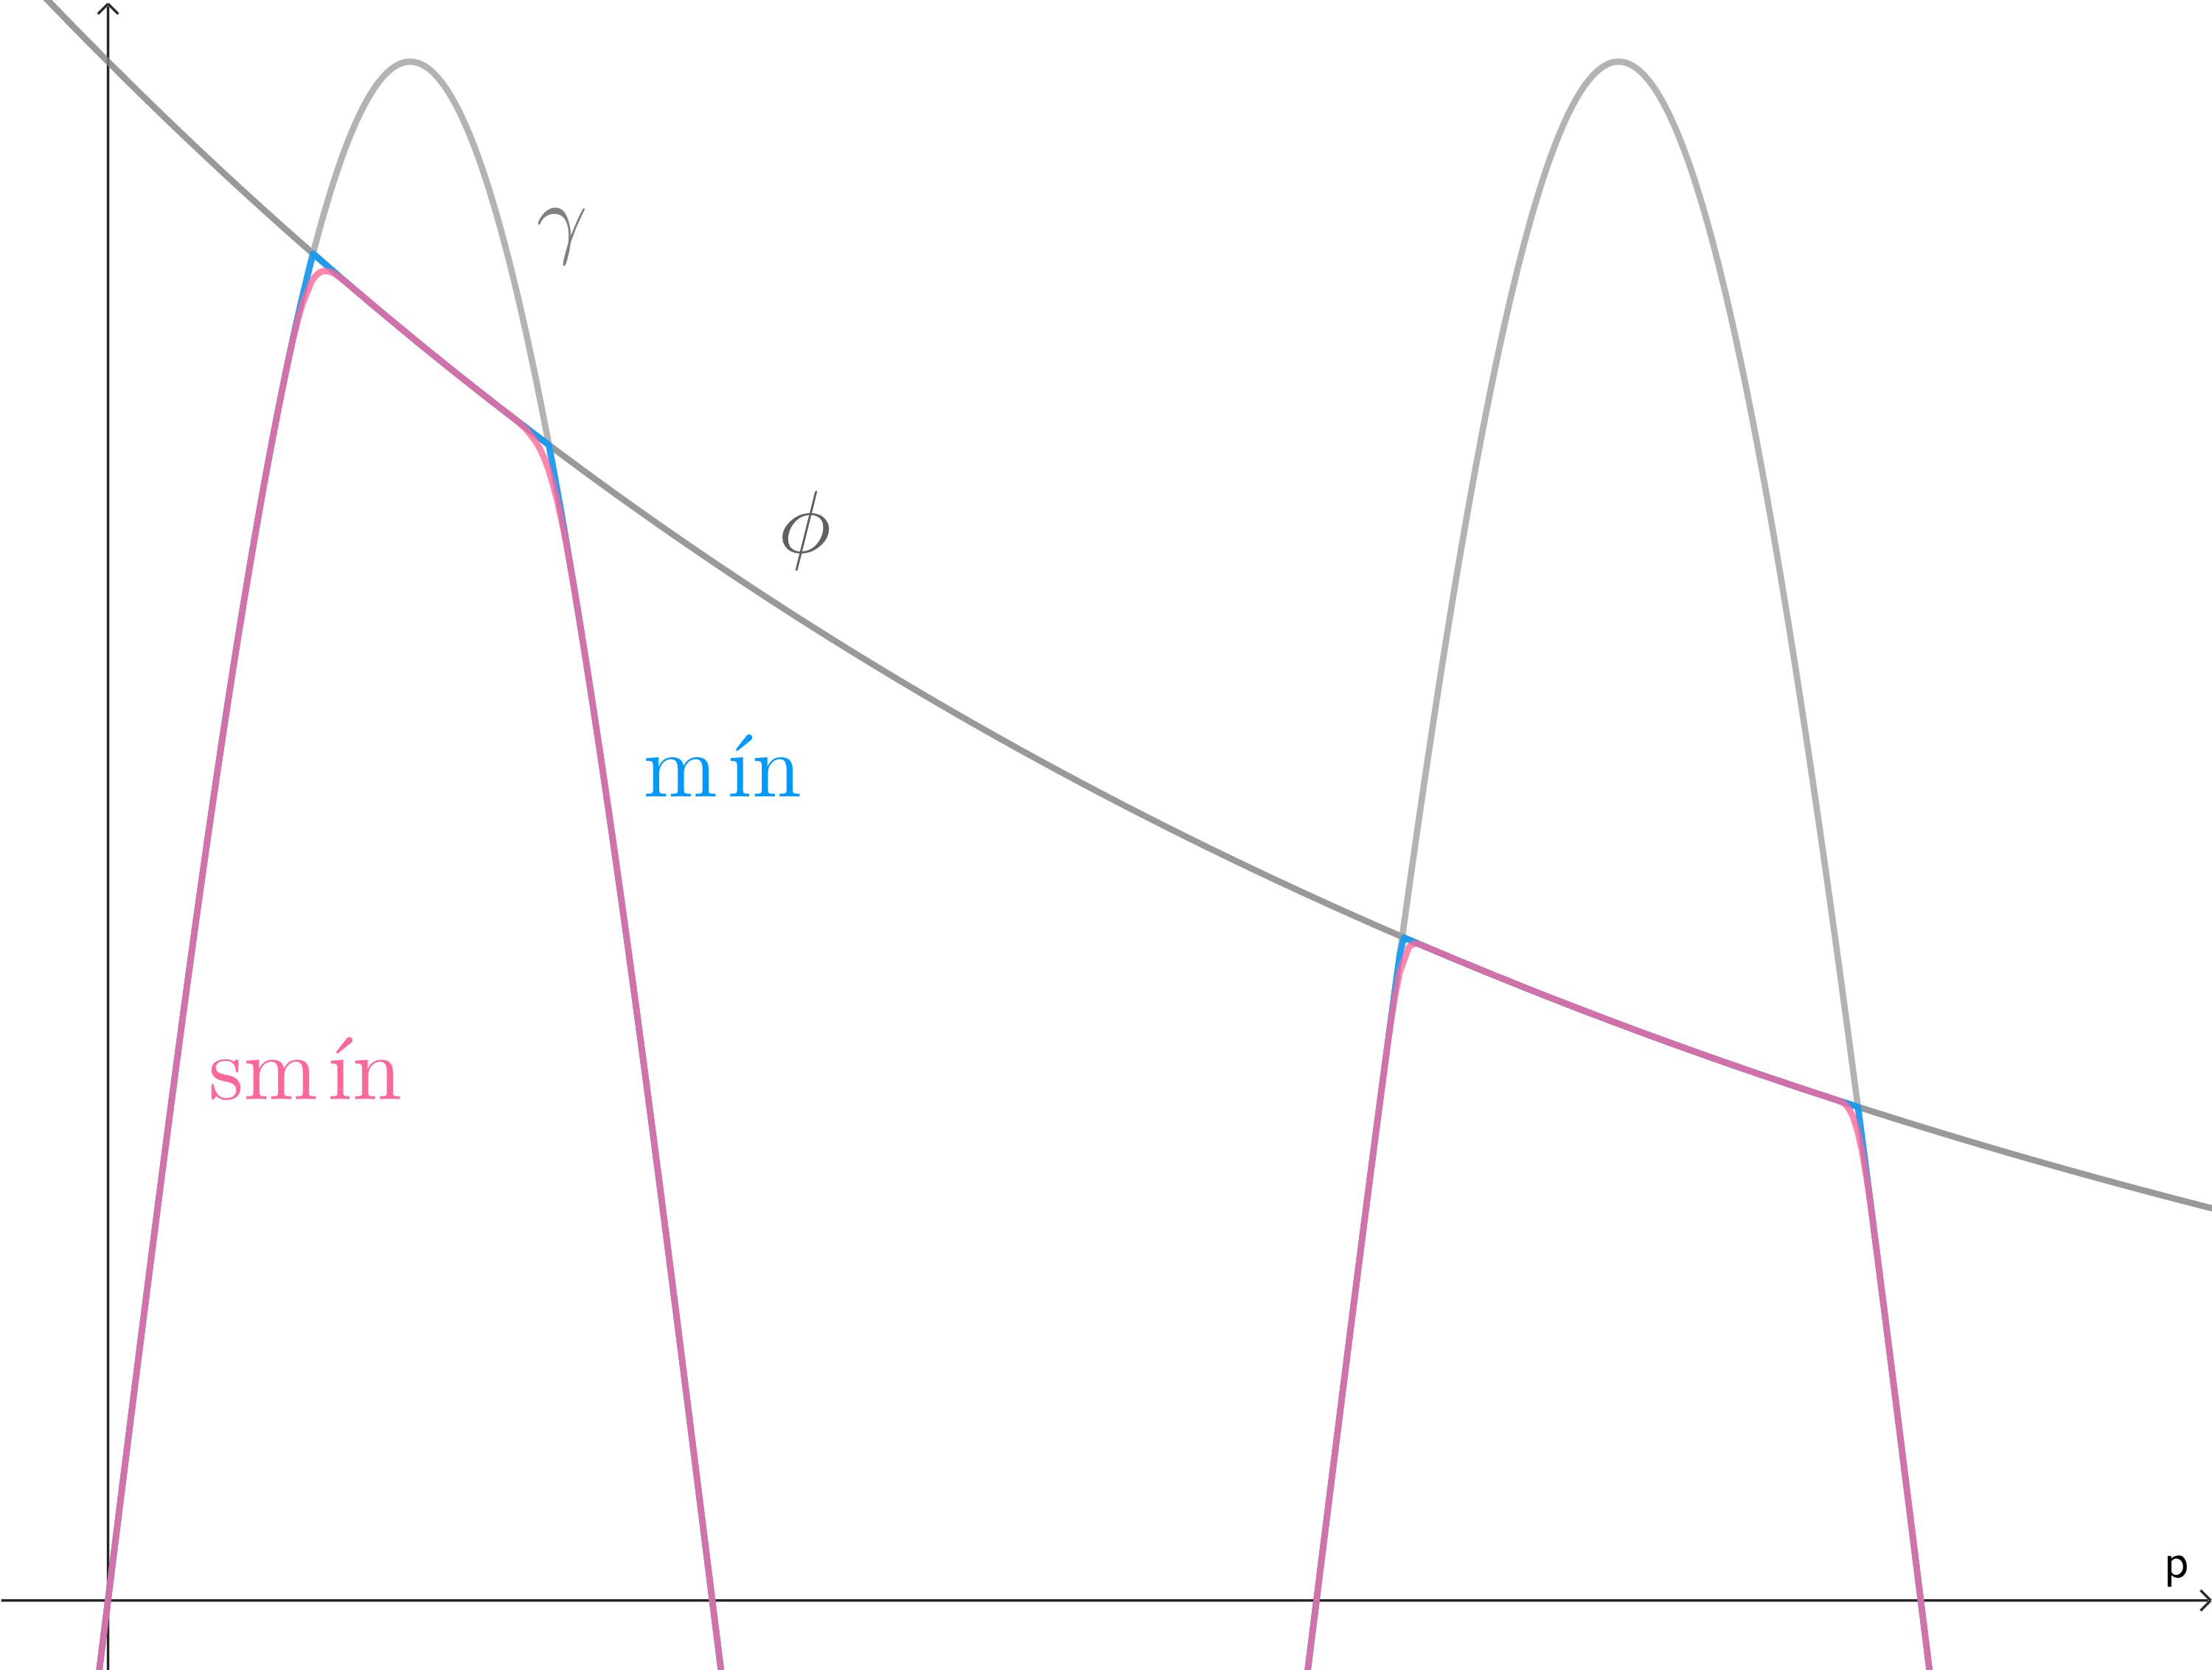
\includegraphics[width=0.95\textwidth]{Plantilla-TFG-master/img/smin_4.png}
        \caption{$k=0.1,\ n=3$}
     \end{minipage}
     \caption{Resultado final de $smin(p)$ }
     \label{fig:smooth2}
\end{figure}





% Por tanto, dadas $\phi$ y $\gamma$, queremos obtener una versión suavizada de $\Min(\phi,\gamma)$ usando interpolación lineal, que llamaremos $\smin$ y tendrá la forma
% \begin{align*}
%           \smin\colon \R^3 &\to \R^3.\\
%           p &\mapsto h(p)\cdot \phi(p) + (1-h(p))\gamma(p) \text{, donde } h \colon \R^3 \to [0,1].
%     \end{align*}


% Pasamos a buscar $h$. Solo queremos modificar la función en los entornos de los puntos en los que intersecan $\phi$ y $\gamma$, de forma que para el resto de puntos debería ser $h=\{0,1\}$. Los puntos de intersección vienen dados como las soluciones de $m(p)=\gamma(p) - \phi(p)$. Podemos además acotar $m(p)$ en el intervalo $[0,1]$ usando $\Min$ y $\Max$, obteniendo un candidato a valor de $h(p)$:
% \begin{equation}
%     \Min\left(\Max\left(\phi(p)-\gamma(p),0\right),1\right) = \Min\left(\Max\left(m(p),0\right),1\right) \in [0,1]
% \end{equation}

% Sin embargo, podemos ver que la interpolación comienza justo en la intersección, mientras que nos gustaría que esto ocurriese antes. Modificamos la expresión anterior para hacer que la intersección sea el punto medio de la interpolación ($h=0.5$):
% \begin{equation}
%    \Min\left(\Max\left(m(p) + \frac{1}{2},0\right),1\right)
% \end{equation}

% Podemos ver los resultados de esta primera aproximación en la \autoref{fig:smooth1}.

% \begin{figure}[!h]
%      \begin{minipage}[c]{0.49\linewidth}
%         \centering
%         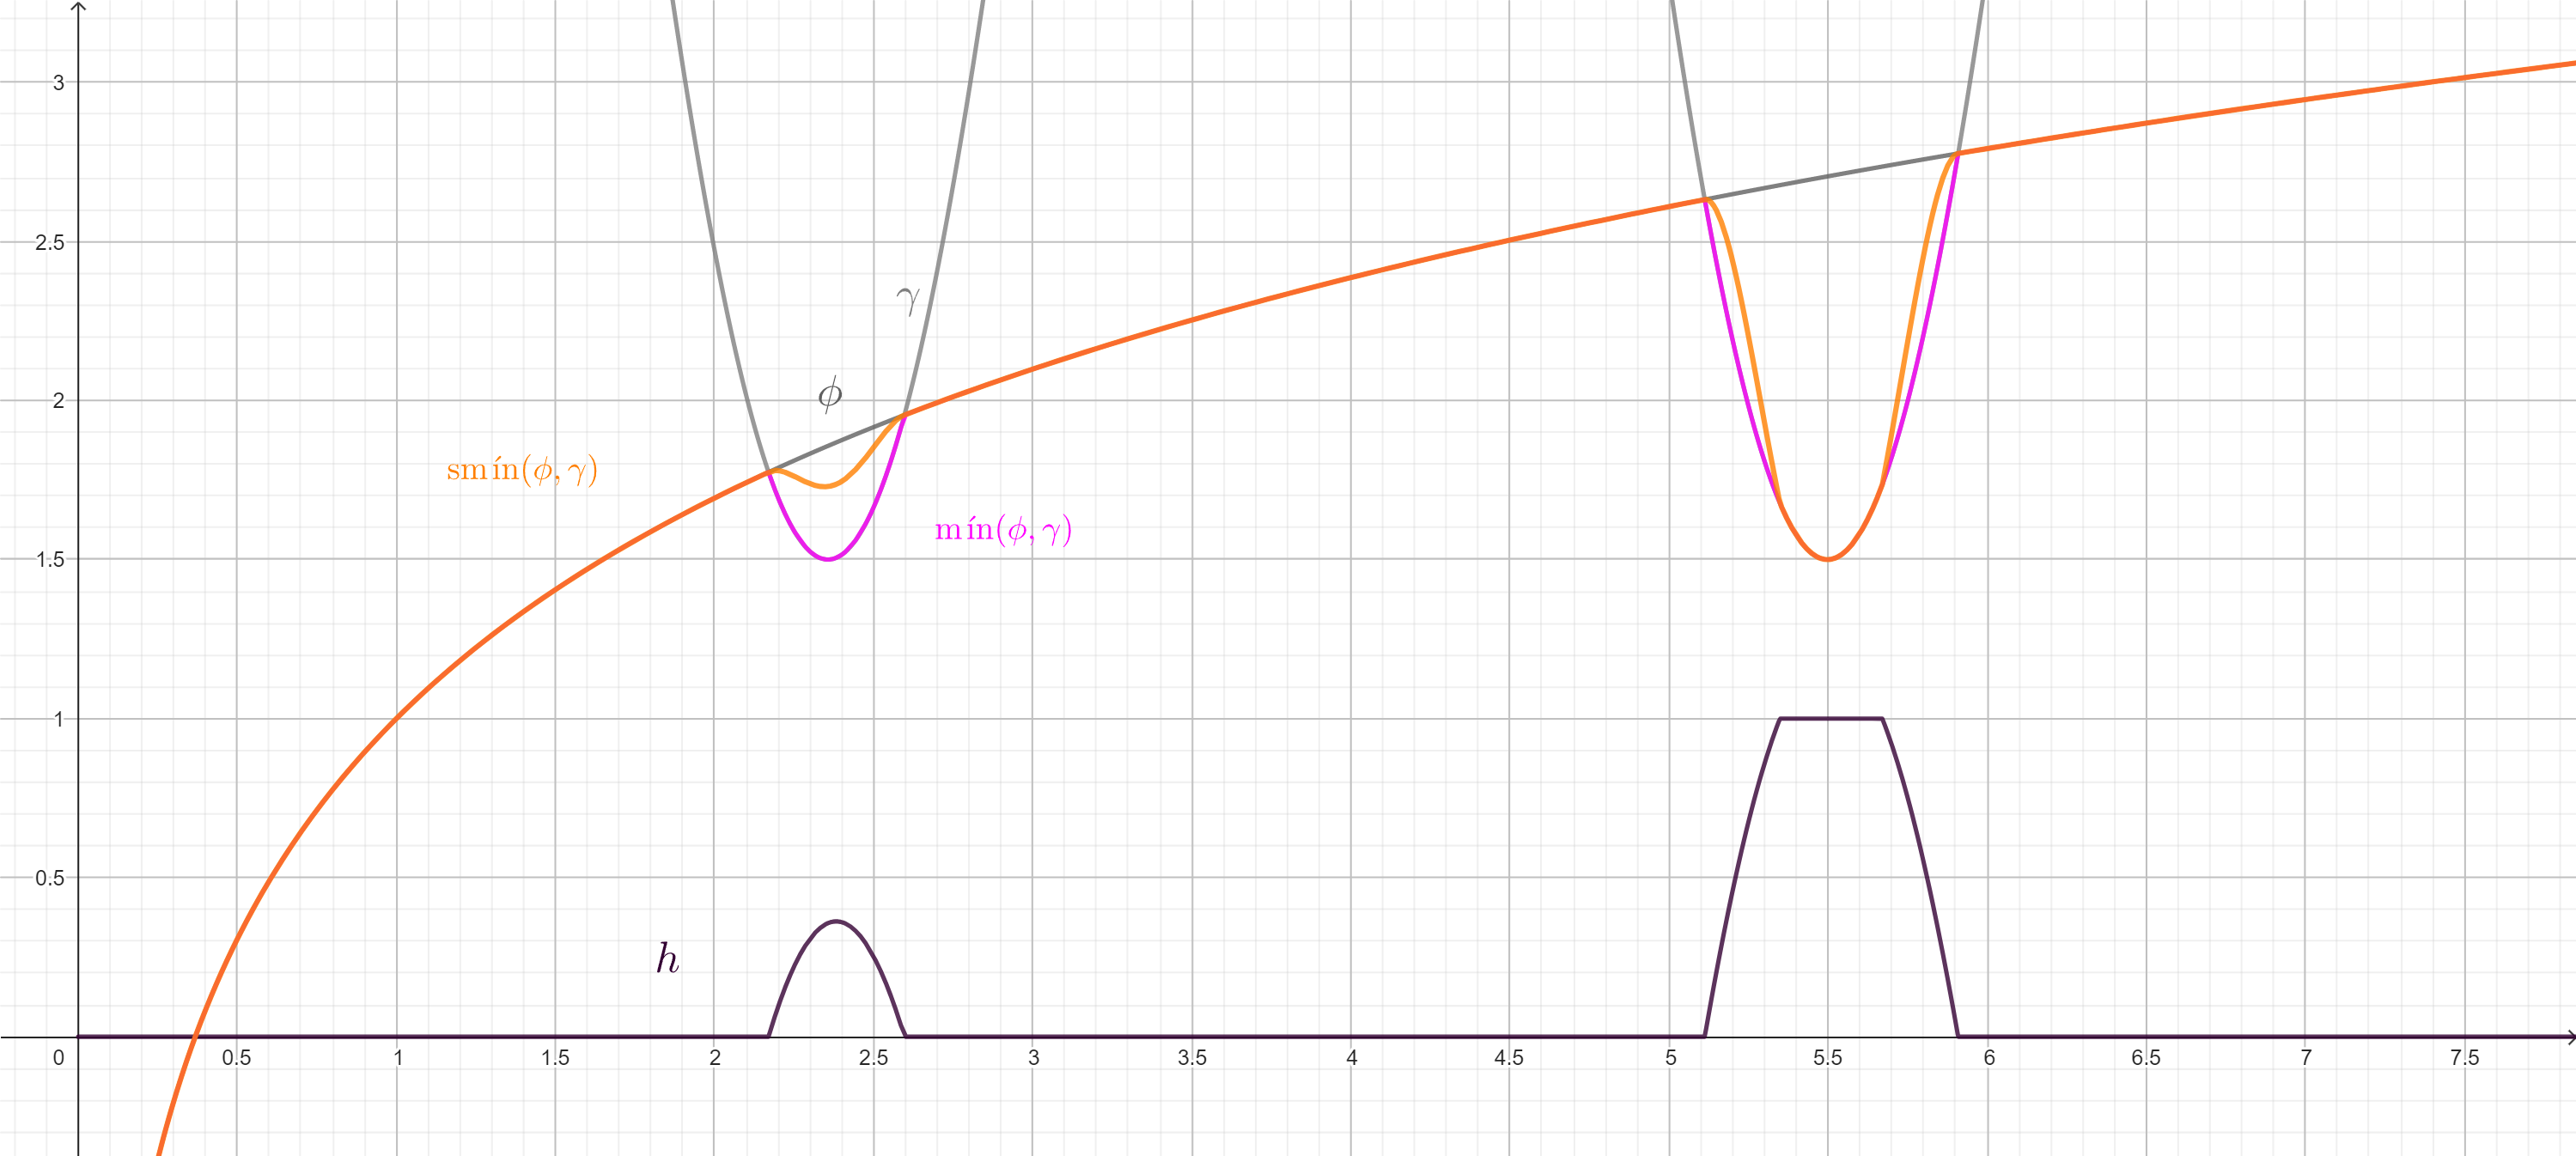
\includegraphics[width=0.95\textwidth]{Plantilla-TFG-master/img/smoothV1_a.png}
%         \caption{$h(p)=0$ en la intersección}
%      \end{minipage}
%      \begin{minipage}[c]{0.49\linewidth}
%         \centering
%         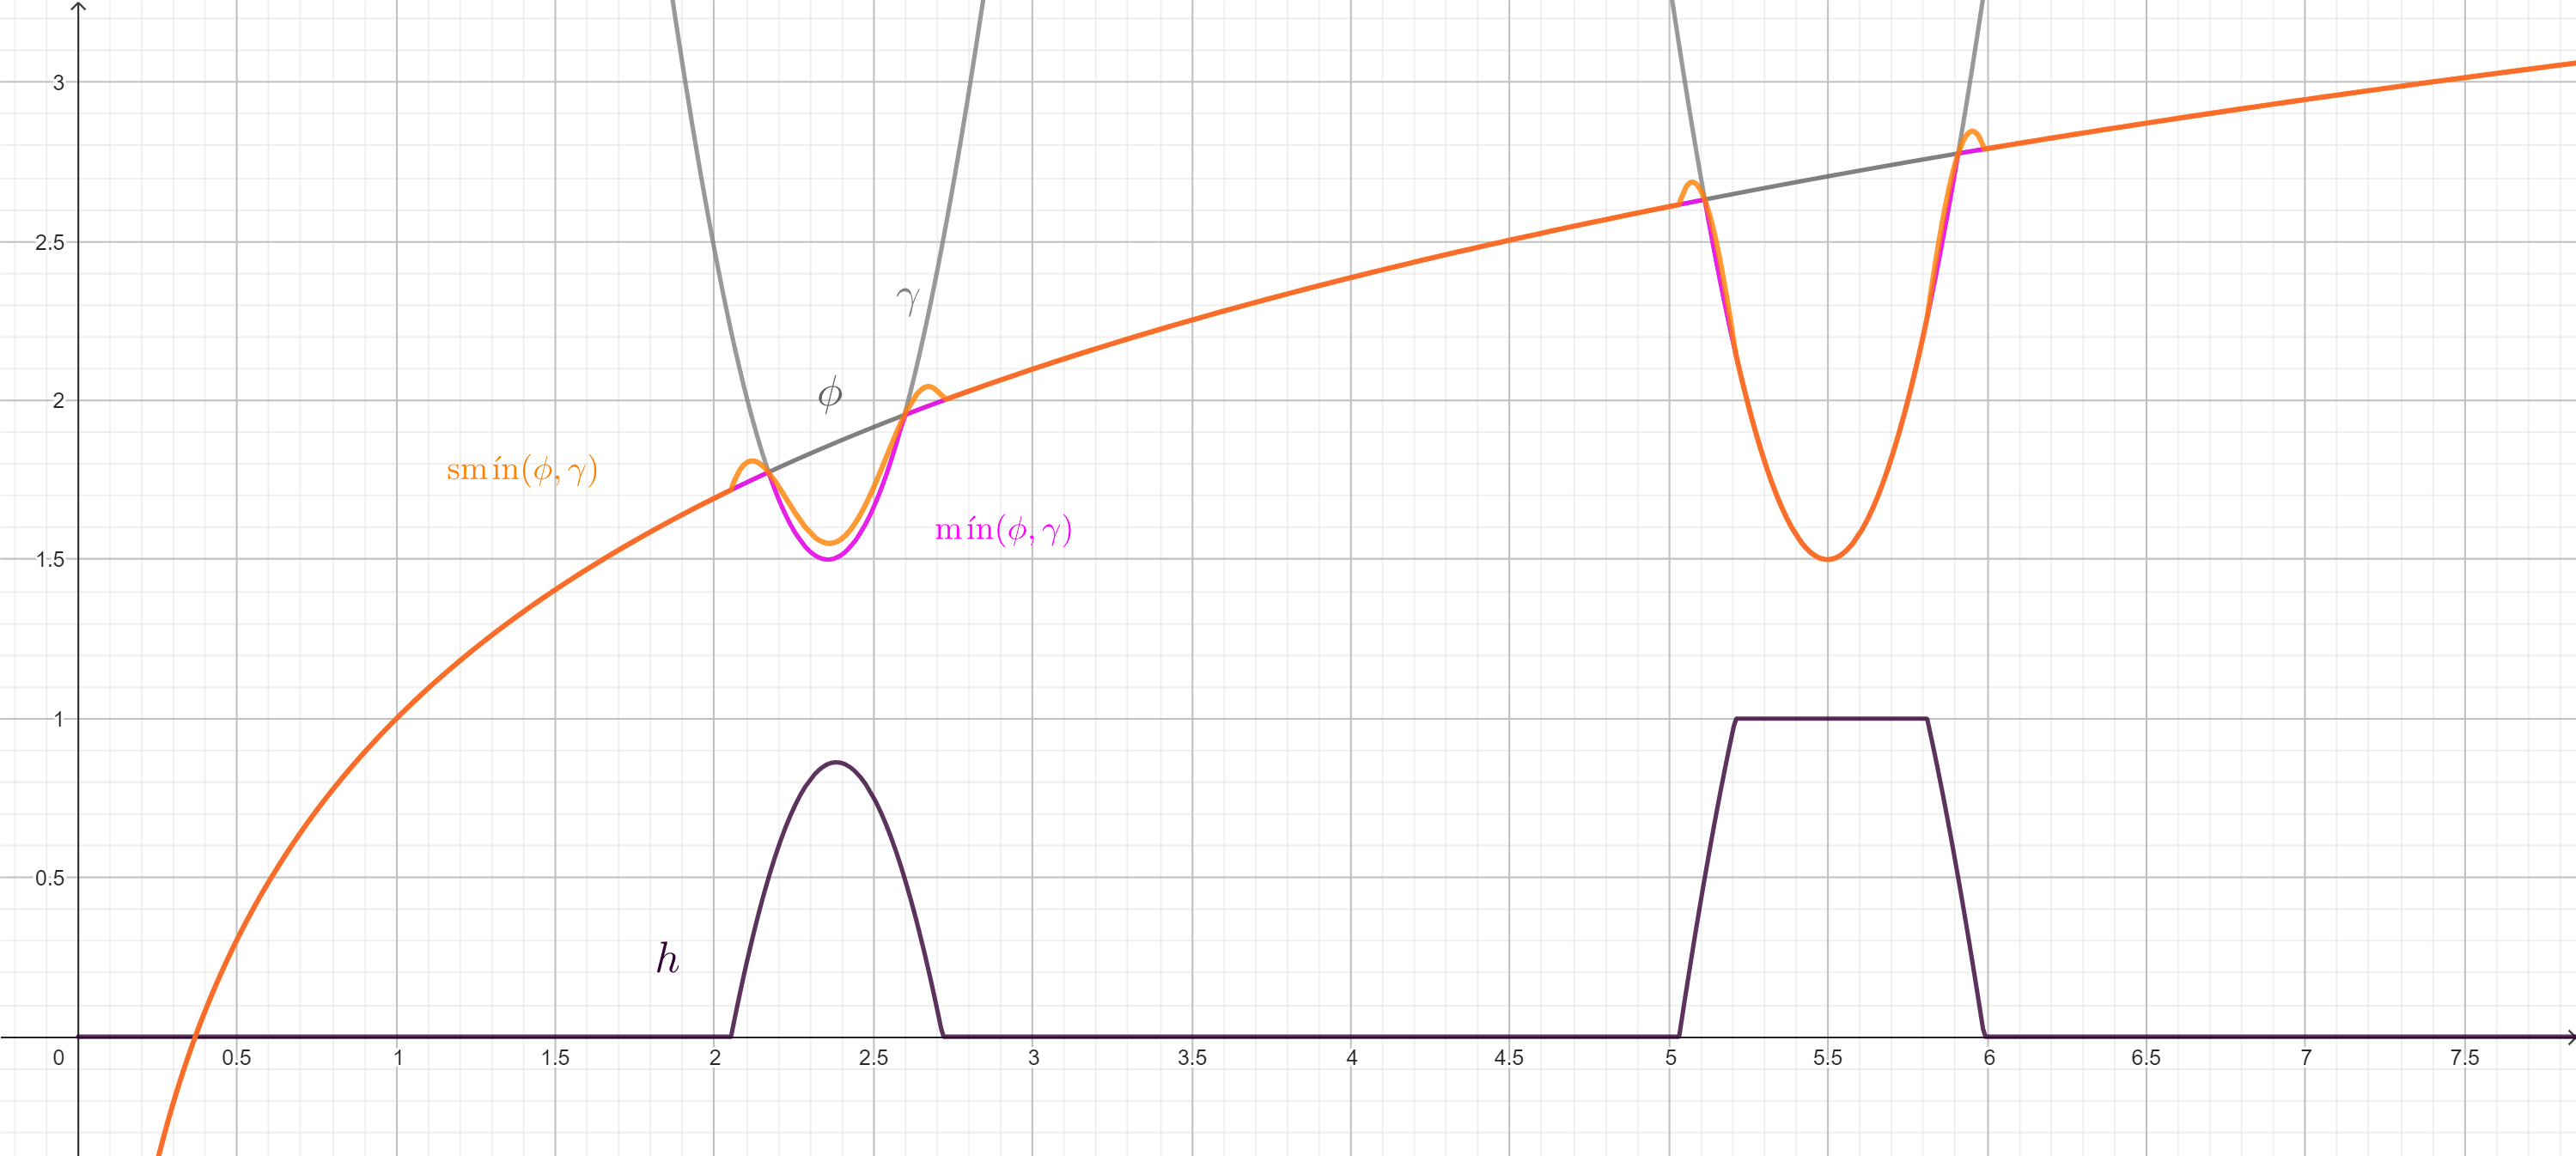
\includegraphics[width=0.95\textwidth]{Plantilla-TFG-master/img/smoothV1_b.png}
%         \caption{$h(p)=0.5$ en la intersección}
%      \end{minipage}
%      \caption{Primera aproximación de la obtención de $h(p)$}
%      \label{fig:smooth1}
% \end{figure}

% Observamos que ahora tenemos un nuevo problema

\begin{definicion}[Operaciones Booleanas Suavizadas]
    Sean $A$ y $B$ isosuperficies generadas por $\phi$ y $\gamma$ respectivamente. La función $\mu$ define la isosuperficie para las siguientes operaciones.
    \begin{itemize}
        \item \textbf{Unión suavizada: } $\mu_{unionS}(p) = \Min(\phi(p),\gamma(p)) - \frac{\Max\left( k - |\phi(p) - \gamma(p)|, 0\right)^n}{2n\cdot k^{n-1}}$.
        \item \textbf{Intersección suavizada: } $\mu_{interS}(p) = -\Min(-\phi(p),-\gamma(p)) + \frac{\Max\left( k - |\phi(p) - \gamma(p)|, 0\right)^n}{2n\cdot k^{n-1}}$.
        \item \textbf{Diferencia suavizada: } $\mu_{difS}(p) = -\Min(-\phi(p),\gamma(p)) + \frac{\Max\left( k - |\phi(p) + \gamma(p)|, 0\right)^n}{2n\cdot k^{n-1}}$.
    \end{itemize}
    La constante $k\in \R^+_0$ controla la influencia del suavizado.        
\end{definicion}

Observamos que los operadores definidos en la \autoref{p:boolean} no son más que un caso particular de estos últimos cuando $k$ tiende a cero. Este método para obtener una versión suavizada de las funciones mínimo y máximo no es el único. Hemos elegido debido a que las funciones obtenidas tienen asociado un coste computacional. Además, su deducción es bastante natural y el efecto que tiene el valor $k$ sobre el resultado final es intuitivo para el usuario. En el artículo que hemos mencionado al inicio de la sección, Íñigo Quílez \cite{article:smooth} presenta otras tres alternativas a esta versión, a la cual él se refiere como \qq{mínimo suavizado polinomial}, y que también son compatibles con \textit{raymarching}.
\begin{itemize}
    \item \textbf{Mínimo suavizado exponencial:} $\smin_{\phi,\gamma}(p) = \frac{-\log_2\left( 2^{-k\phi(p)} + 2^{-k\gamma(p)} ) \right)}{k}$.
    \item \textbf{Mínimo suavizado potencial:} $\smin_{\phi,\gamma}(p) = \left(\frac{\phi(p)^k \cdot \gamma(p)^k}{\phi(p)^k + \gamma(p)^k}\right)^{1/k}$.
    \item \textbf{Mínimo suavizado por raíz:} $\smin_{\phi,\gamma}(p) = \frac{\phi(p) + \gamma(p) - \sqrt{(\phi(p)-\gamma(p))^2+k}}{2}$.
\end{itemize}

La principal ventaja de la versión polinomial respecto a estas es que es la más rápida al ser sus cálculos computacionalmente más baratos. Por otro lado tanto la exponencial como la potencial permiten ser adaptadas fácilmente para calcular el mínimo de un conjunto arbitrario de puntos, útil cuando se trabaja con patrones de voronoi o nubes de puntos. Además, la versión exponencial produce siempre el mismo resultado independientemente del orden en el que se aplique. Es decir,
\begin{equation*}
    \smin_{a,\smin_{b,c}} = \smin_{b,\smin_{a,c}}.
\end{equation*}

En la \autoref{fig:smoothVS} podemos ver un ejemplo de uso de estas versiones, en las que además se ha usado el valor de $w_k$ de la ecuación \autoref{eq:correccion} para interpolar la componente difusa de ambas primitivas usando el método \texttt{mix} de GLSL. Como vemos, no hay diferencias notables entre las distintas versiones, así que nos quedaremos con el método más eficiente: el polinómico.
\begin{figure}[htbp]
    \centering
    \begin{subfigure}[b]{0.25\textwidth}
        \centering
        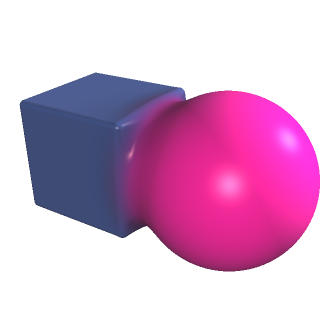
\includegraphics[width=\textwidth]{Plantilla-TFG-master/img/unionMethodOG.png}
        \caption{Polinomial, $k=1.5$}
    \end{subfigure}
    \hfill
    \begin{subfigure}[b]{0.25\textwidth}
        \centering
        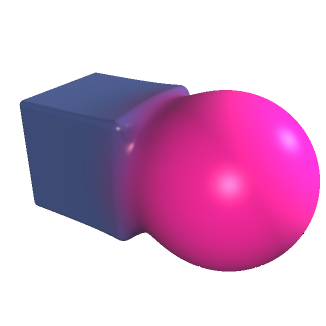
\includegraphics[width=\textwidth]{Plantilla-TFG-master/img/unionMethodExp.png}
        \caption{Exponencial, $k=2.5$}
    \end{subfigure}
    \hfill
    \begin{subfigure}[b]{0.25\textwidth}
        \centering
        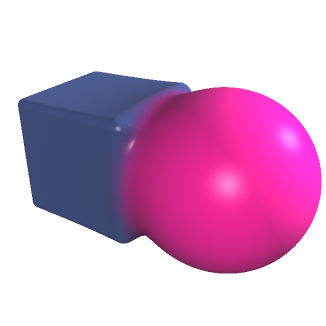
\includegraphics[width=\textwidth]{Plantilla-TFG-master/img/unionMethodRoot.png}
        \caption{Raíz, $k=1$}
    \end{subfigure}
    
    \caption{Diferentes versiones de la unión suavizada}
    \label{fig:smoothVS}
\end{figure}

\subsection{Operaciones afines}
Pasamos ahora a estudiar otro tipo de operaciones que nos permitirán aplicar movimientos rígidos y cambios de escala a las primitivas en la escena. A diferencia de los operadores booleanos, que eran binarios, estas operaciones se aplican a una única primitiva. Su funcionamiento se basará en aplicar una transformación $t:\R^3\to \R^3$ a cada punto de la isosuperficie $S_{\phi}$ para obtener la transformada $S_{\gamma}$. Si queremos saber si un punto $q\in\R^3$ está en $S_{\gamma}$, tenemos que comprobar si su preimagen por la transformación pertenece a $S_{\phi}$. Por tanto, bastará evaluar la SDF original en $t^{-1}(p)$:
\begin{equation*}
    \gamma(p) = \phi(t^{-1}(p)).
\end{equation*}

Este razonamiento funciona bien para transformaciones como las traslaciones o rotaciones, que son movimientos rígidos y mantienen las distancias. Sin embargo, este no es el caso del escalado, ya que si tomamos $l(p) = sp$ con $s\in \R^+_0$
\begin{equation*}
    \Vert p-p'\Vert = d, \text{ luego }  \Vert l(p)-l(p')\Vert = \Vert sp-sp'\Vert = s\Vert p-p'\Vert = s\cdot d,\  \text{ donde } p,p' \in S_{\phi}.
\end{equation*}
Como las distancias se escalan, deberemos hacer lo propio con la función que genere la nueva isosuperficie, aplicándole el mismo factor de escalado $s$ como muestra la \autoref{d:afines}.

\begin{definicion}[Operaciones afines]\label{d:afines}
    Sea $A$ una isosuperficie. Definimos las SDFs para las siguientes operaciones.
    \begin{itemize}
        \item \textbf{Traslación de vector $\boldsymbol{v\in R^3}$: } $\sdf_{traslacion}(p) = \sdf_{A}(p - v)$.
        \item \textbf{Escalado uniforme de dimensiones $\boldsymbol{(s,s,s)\in \R^3}$: } $\sdf_{escalado}(p) = \sdf_{A}(p/s)\cdot s$.
        \item \textbf{Rotaciones de ángulo $\boldsymbol{\alpha\in \R}$ sobre los ejes $\boldsymbol{x,y,z}$: }
        \begin{align*}
            \sdf_{rotX}(p) &= \mu_{A}(R_x^{-1}(\alpha)\cdot p^t),\ \text{donde } R_x(\alpha) = 
            \begin{pmatrix}
                1&0&0\\
                0&\cos(\alpha) & -\sin(\alpha) \\
                0&\sin(\alpha) & \cos(\alpha) 
                \end{pmatrix},\\[10pt] 
            \sdf_{rotY}(p) &= \mu_{A}(R_y^{-1}(\alpha)\cdot p^t),\ \text{donde } R_y(\alpha) = \begin{pmatrix}
            \cos(\alpha) &0& \sin(\alpha)\\
            0&1&0\\
            -\sin(\alpha) &0& \cos(\alpha) 
            \end{pmatrix},\\[10pt]
            \sdf_{rotZ}(p) &= \mu_{A}(R_z^{-1}(\alpha)\cdot p^t),\ \text{donde } R_z(\alpha) = \begin{pmatrix}
            \cos(\alpha) & -\sin(\alpha) & 0\\
            \sin(\alpha) & \cos(\alpha) & 0\\
            0&0&1
            \end{pmatrix}.
        \end{align*}
    \end{itemize}
\end{definicion}

Observamos que en este caso sí que obtenemos funciones distancia con signo como resultado, al contrario de lo que ocurría con las operaciones booleanas.
\begin{figure}[ht!]
    \centering
    \begin{subfigure}[b]{0.24\textwidth}
        \centering
        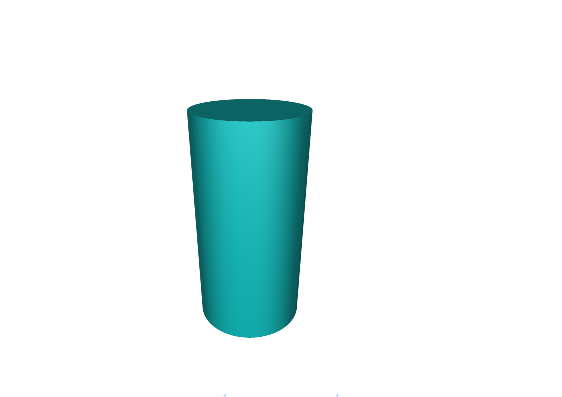
\includegraphics[width=\textwidth]{Plantilla-TFG-master/img/afin_og.png}
        \caption{Original}
    \end{subfigure}
    \hfill
    \begin{subfigure}[b]{0.24\textwidth}
        \centering
        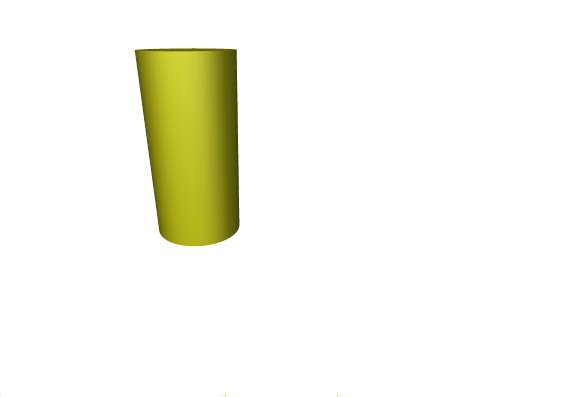
\includegraphics[width=\textwidth]{Plantilla-TFG-master/img/afin_trans.png}
        \caption{Traslación}
    \end{subfigure}
    \hfill
    \begin{subfigure}[b]{0.24\textwidth}
        \centering
        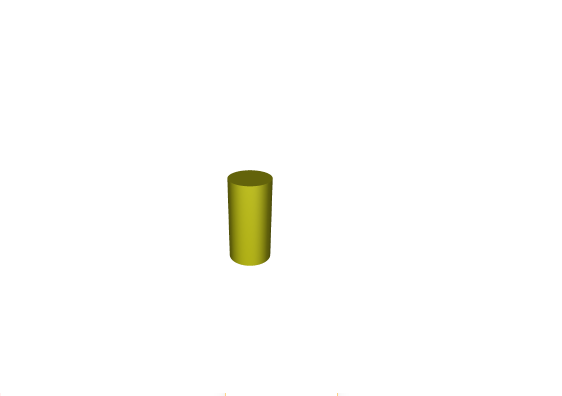
\includegraphics[width=\textwidth]{Plantilla-TFG-master/img/afin_scale.png}
        \caption{Escalado uniforme}
    \end{subfigure}
    \hfill
    \begin{subfigure}[b]{0.24\textwidth}
        \centering
        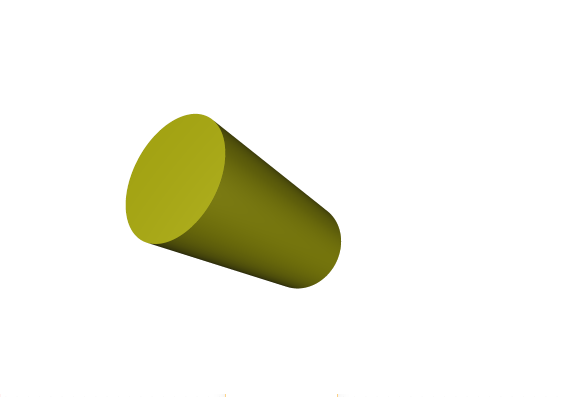
\includegraphics[width=\textwidth]{Plantilla-TFG-master/img/afin_rot.png}
        \caption{Rotación}
    \end{subfigure}
    \hfill
   
    \caption{Ejemplos de uso de los operadores afines}
\end{figure}

\subsection{Operaciones deformantes}
Siguiendo el mismo razonamiento, podemos definir operaciones que modifiquen la geometría de la superficie aplicando rotaciones o traslaciones al punto en el que se evalúa la función distancia con signo original. De esta forma podemos obtener operadores que de otra forma sería mucho más complicado implementar, como la torsión o el redondeo de los bordes de una primitiva \cite{deform}.

\begin{definicion}[Operaciones Deformantes]
    Sea $A$ una isosuperficie. La función $\mu$ define la isosuperficie para las siguientes operaciones.
    \begin{itemize}
        
        \item \textbf{Torsión: } $\mu_{torsion}(p) = \sdf_{A}(p')$, con $p' = R_z(ky)\cdot (x,z,y)^t$.
        \item \textbf{Plegado: } $\mu_{plegado} =\sdf_{A}(p')$, con $p' = R_z(kx)\cdot p^t$.
        \item \textbf{Redondeo: } $\mu_{redondeo}(p) = \sdf_{A}(p) - k$.
        \item \textbf{Desplazamiento: } $\mu_{desplazamiento}(p) = \sdf_{A}(\delta(p))$.
        \item \textbf{Elongación de tamaño $\boldsymbol{h\in \R^3}$: } $\sdf_{elongacion}(p) = \mu_{A}(p')$, con $p' = p - c(p, -h, h)$.
    \end{itemize}
    En estas definiciones,
    \begin{itemize}
        \item $k\in \R^+_0$ controla la intensidad de la deformación,
        \item $\delta\colon \R^3\to \R^3$ es un patrón de desplazamiento,
        \item $R_z(\alpha)\in \mathcal{M}_3(\R)$ es la matriz de rotación de ángulo $\alpha$ sobre el eje $z$ dada en la \autoref{d:afines},
        \item $c\colon \R^3\times \R^3 \times \R^3 \to \R^3,\ c(x,a,b)$ acota cada componente de $x$ entre las de $a$ y $b$.
    \end{itemize}
\end{definicion}

Las únicas operaciones que nos proporcionan una función distancia con signo como resultado son el redondeo y la elongación. El resto es recomendable usarlas lo menos posible, pues las isosuperficies que generan pueden presentar fallos al ser renderizadas.
\begin{figure}[ht!]
    \centering
    \begin{subfigure}[b]{0.30\textwidth}
        \centering
        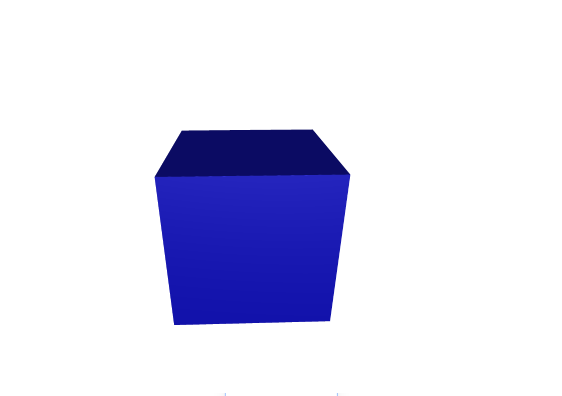
\includegraphics[width=\textwidth]{Plantilla-TFG-master/img/deform_og.png}
        \caption{Original}
    \end{subfigure}
    \hfill
    \begin{subfigure}[b]{0.30\textwidth}
        \centering
        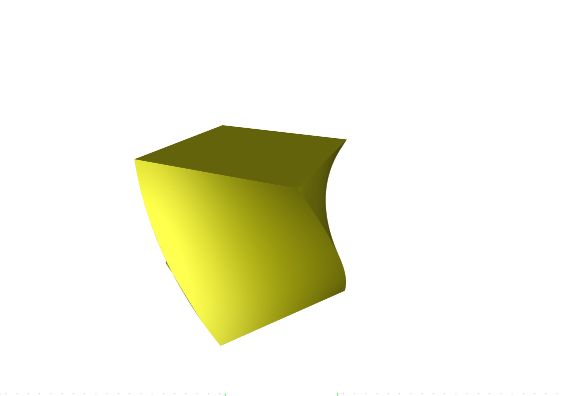
\includegraphics[width=\textwidth]{Plantilla-TFG-master/img/deform_twist.png}
        \caption{Torsión}
    \end{subfigure}
    \hfill
    \begin{subfigure}[b]{0.30\textwidth}
        \centering
        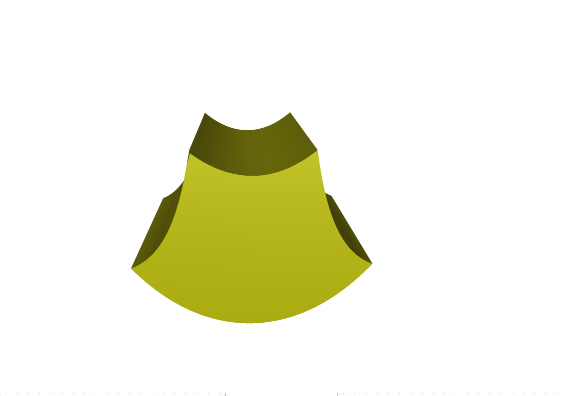
\includegraphics[width=\textwidth]{Plantilla-TFG-master/img/deform_bend.png}
        \caption{Plegado}
    \end{subfigure}
    \hfill
    \begin{subfigure}[b]{0.30\textwidth}
        \centering
        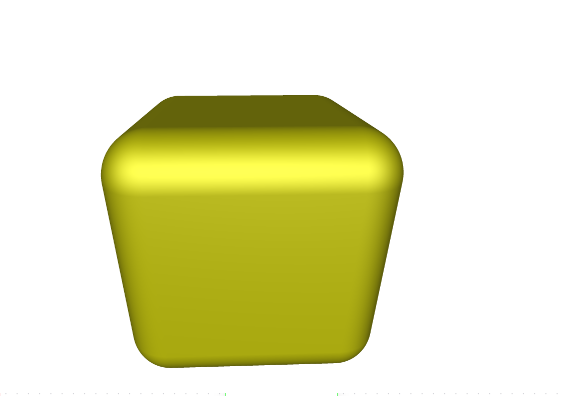
\includegraphics[width=\textwidth]{Plantilla-TFG-master/img/deform_round.png}
        \caption{Redondeo}
    \end{subfigure}
    \hfill
    \begin{subfigure}[b]{0.30\textwidth}
        \centering
        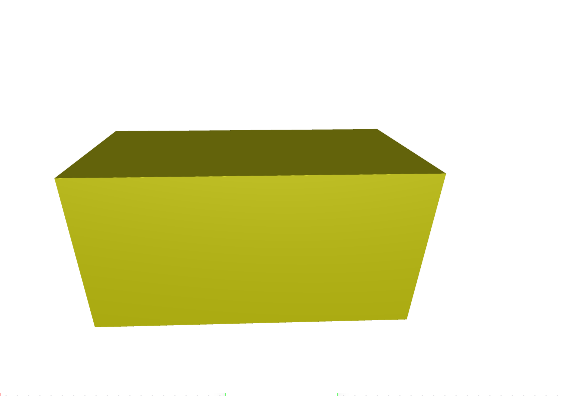
\includegraphics[width=\textwidth]{Plantilla-TFG-master/img/deform_elong.png}
        \caption{Elongación}
    \end{subfigure}
    
    \caption{Ejemplos de uso de los operadores de deformación}
\end{figure}

\subsection{Operaciones de repetición}
También podemos usar la técnica de cambiar el punto en el que evaluamos la función distancia para, en lugar de modificar la geometría original, añadir copias de la primitiva identificando varios puntos con uno que pertenezca a la isosuperficie. La manera más inmediata de conseguir esto es a través de la función valor absoluto, que nos permitirá identificar la componente de cada punto con su opuesta para generar simetrías, y el operador módulo, que identificará puntos a una distancia fija en cada eje.

\begin{definicion}[Operadores de Posicionamiento]\label{d:posicionamiento}
    Sea $A$ una isosuperficie. La función $\mu$ define la isosuperficie para las siguientes operaciones.
    \begin{itemize}
        \item \textbf{Simetrías sobre los ejes $\boldsymbol{x,y,z}$:}
        \begin{gather*}
            \mu_{simX}(p) = \sdf_{A}(\vert x\vert, y, z),\quad \mu_{simY}(p) = \sdf_{A}(x, \vert y\vert,  z),\\[5pt] \mu_{simZ}(p) = \sdf_{A}(x,y,\vert z\vert).
        \end{gather*}
        \item \textbf{Simetrías sobre los planos $\boldsymbol{xy,xz,yz}$:}
        \begin{gather*}
            \mu_{simXY}(p) = \sdf_{A}(\vert x\vert, \vert y\vert, z),\quad \mu_{simXZ}(p) = \sdf_{A}(\vert x\vert, y,  \vert z\vert),\\[5pt]\mu_{simYZ}(p) = \sdf_{A}(x,\vert y\vert ,\vert z\vert).
        \end{gather*}
        \item \textbf{Repetición $\boldsymbol{l\in \N^3}$ veces en los ejes $\boldsymbol{x,y,z}$ con separación $\boldsymbol{s\in\R}$:} 
        \begin{equation*}
            \mu_{rep}(p) = \sdf_{A}(p - s\cdot c\left(r\left(\frac{p}{s}\right), -l, l\right).
        \end{equation*}
        \item \textbf{Repetición infinita:}
        \begin{equation*}
            \mu_{repInf}(p) = \sdf_{A}\left((p+\frac{l}{2}\mod l )- \frac{l}{2}\right).
        \end{equation*}
    \end{itemize}
    En estas definiciones,
    \begin{itemize}
        \item $c\colon \R\times\R\times\R\to \R,\ c(x,a,b) = \Min(\Max(x, a), b)$ acota $x$ en $[a,b]$,
        \item $r\colon \R^3 \to \R^3$ redondea las componentes de un vector a sus enteros más cercanos.
    \end{itemize}
\end{definicion}
\begin{figure}[ht!]
    \centering
    \begin{subfigure}[b]{0.48\textwidth}
        \centering
        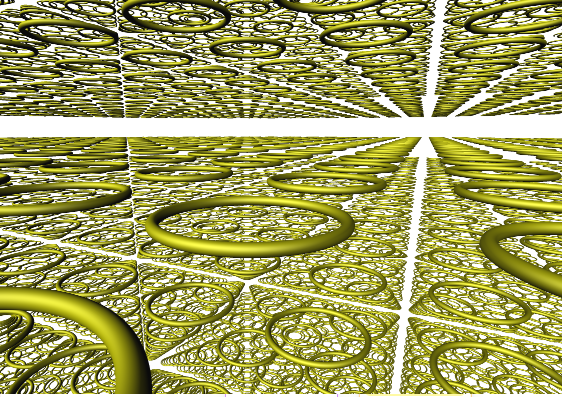
\includegraphics[width=\textwidth]{Plantilla-TFG-master/img/rep.png}
        \caption{Repetición infinita}
    \end{subfigure}
    \hfill
    \begin{subfigure}[b]{0.48\textwidth}
        \centering
        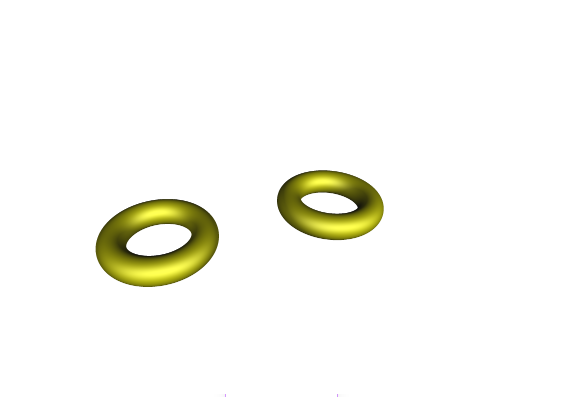
\includegraphics[width=\textwidth]{Plantilla-TFG-master/img/sym.png}
        \caption{Simetría}
    \end{subfigure}
    \hfill
        
    \caption{Ejemplos de uso de los operadores de repetición}
\end{figure}

Las funciones obtenidas no son en general funciones distancia con signo. Esto ocurre en los siguientes casos.
\begin{itemize}
    \item Al aplicar simetrías, cuando el objeto interseca el plano de simetría.
    \item En el caso de la repetición infinita, cuando las dimensiones del objeto sean mayores o iguales a $l/2$.
    \item Siempre para la repetición finita, como consecuencia de usar la función máximo. 
\end{itemize}

No obstante, este tipo de operaciones evidencia el potencial que tienen las funciones distancia con signo en cuanto a eficiencia a la hora de generar nuevas superficies, ya que podemos visualizar miles de objetos al precio de uno. Por ejemplo, podríamos generar un campo de césped a partir de una única brizna de hierba, o modelar solo una fracción de un objeto y generar el resto usando simetrías.

